\chapter{Estado de la cuestión}
\label{chap:antecedentes}

\drop{E}{}n este capítulo se lleva a cabo una prospección de los sistemas y artículos
que se han efectuado hasta la fecha, de modo que se contextualice el \acs{TFG} en el ámbito 
de la utilización de \acs{UAV}s, en diferentes entornos de la ingeniería civil en general y, más
concretamente, en situaciones de emergencia. Asimismo se analizarán las tecnologías de mayor 
relevancia para el desarrollo e implementación del sistema adaptativo.  

\section{Vehículo aéreo no tripulado}
\label{sec:vehiculonotripulado}

La aviación no tripulada comprende una amplia gama de aeronaves. El origen de estas aeronaves no tripuladas reside 
en la creación de los torpedos aéreos, que después evolucionaron a través de las bombas guiadas, los blancos 
aéreos (o drones), los señuelos, los modelos deportivos de radiocontrol, las aeronaves de investigación, 
las aeronaves de reconocimiento y las aeronaves de combate.

Un \acs{UAV} es «un vehículo aéreo motorizado \textbf{i)} que no lleva a bordo a un operador humano, 
\textbf{ii)} que utiliza las fuerzas aerodinámicas para proporcionar la elevación del vehículo, \textbf{iii)} que puede volar autónomamente 
o ser tripulado por control remoto, \textbf{iv)} que puede ser sustituido o recuperado, y \textbf{v)} que puede transportar una 
carga letal o no» \cite{UAV}. Dada esta definición quedan excluidos:

\begin{itemize}
\item Los planeadores, debido a que no usan una planta propulsora.
\item Los globos y dirigibles, ya que no se elevan mediante fuerzas aerodinámicas sino mediante fuerzas de flotabilidad.
\item Los misiles balísticos, misiles de crucero y proyectiles de artillería.
\end{itemize}

La palabra \acs{UAV} se comienza a hacer frecuente en los años 90 para representar a las aeronaves robóticas 
y así, reemplazar el término vehículo aéreo pilotado remotamente o \acs{RPV}. \acs{UAV} y \acs{RPV} no son más 
que dos nombres entre aproximadamente la docena que han recibido las aeronaves robóticas no tripuladas a lo largo de la historia (ver Figura~\ref{fig:cronologia}).

«En el año 2011 la Organización de Aviación Civil Internacional, organismo especializado de las Naciones 
Unidas para la aviación civil y del cual España forma parte al haber suscrito el Convenio de Chicago de 1944, 
publicó su Circular 328 en la cual por vez primera reconoce a las aeronaves no tripuladas como aeronaves, 
con todo lo que ello trae consigo, y de entre todas las posibles tipologías escoge a las que se pilotan de manera 
remota para ser consideradas como aptas para la aviación civil» \cite{dron1}. Así es como se acuñan los términos que a continuación se detallan, y que en la actualidad tienen una validez internacional y practicamente única en todos los ámbitos. Estos términos son:

\begin{itemize}
\item \textbf{Aeronave pilotada remotamente} o \textbf{\acs{RPA}}: aeronave en la que el piloto al mando no está a bordo.
\item \textbf{Sistema de aeronave pilotada remotamente} o \textbf{\acs{RPAS}}: conjunto de elementos configurables formado por un \acs{RPA}, 
una estación de pilotaje remoto asociada o \acs{RPS}, un sistema de enlace de mando y cualquier otro elemento requerido en cualquier 
punto durante la operación del vuelo.
\end{itemize}

\begin{figure}[!h]
\begin{center}
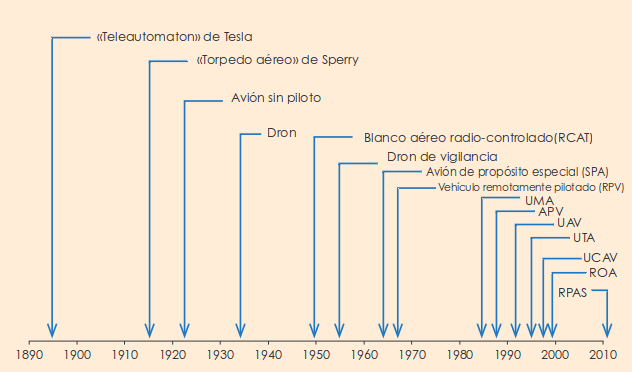
\includegraphics[width=0.8\textwidth]{/cronologia1.jpg}
\caption[Cronología de los nombres aplicados a las aeronaves robóticas]{Cronología de los nombres aplicados a las aeronaves robóticas \footnotemark}
\label{fig:cronologia}
\end{center}
\end{figure}

\footnotetext{Los acrónimos no especificados se corresponden con: UMA = Unmanned Aircraft, 
APV = Automatically Piloted Vehicle, UTA = Unmanned Tactical Aircraft, UCAV = Unmanned Combat Air Vehicle, 
ROA = Remotely Operated Aircraft.}

\subsection{Nacimiento y desarrollo de aeronaves pilotadas por control remoto}
\label{sec:historia}

Los europeos fueron pioneros en concebir los principios de la aeronáutica y, al 
tratar de emplearlos en aeronaves, volaron modelos no tripulados que pueden ser los primeros vehículos 
aéreos no tripulados de la historia. Precursores de la aviación en distintos países siguieron una progresión que va de los
planeadores a los aviones propulsados no tripulados, y de los vuelos no tripulados a los
tripulados (ver Cuadro~\ref{tab:pioneros}). Su limitación tecnológica, no disponer de un motor con suficiente relación potencia-peso, 
impidió que sus diseños pudieran mantenerse en el aire.

\begin{table}[htbp]
  \centering
  {\small
  \begin{tabular}{p{.1\textwidth}p{.2\textwidth}p{.18\textwidth}p{.17\textwidth}p{.2\textwidth}}
  \tabheadformat
  \tabhead{País} &
  \tabhead{Planeador no tripulado} &
  \tabhead{Planeador tripulado} &
  \tabhead{Avión no tripulado}  &
  \tabhead{Avión tripulado}	\\
\hline
\textit{Inglaterra}  & Cayley, 1809 & Cayley, 1849 & Cody, 1907 & Cody, 1908 \\
                 
\hline
\textit{Francia} &  & Ferber, 1901 & Du Temple, 1857 & Santos-Dumont, 1906 \\
                       
\hline
\textit{Alemania}  &  & Lilienthal, 1891 &  &  \\
                       
\hline
\textit{Japón}  &  & Leprieur/Aibara, 1909 & Ninomiya, 1891 & Nagahara, 1911 \\
                      
\hline
\textit{Rusia}  &  &  &  & Rossinsky, 1910 \\
                   
\hline
\textit{Estados Unidos}  &  & Chanute, 1896 & Langley, 1896 & Hnos. Wright, 1903  \\
                      
\hline
\end{tabular}


% Local variables:
%   coding: utf-8
%   ispell-local-dictionary: "castellano8"
%   TeX-master: "main.tex"
% End:

  }
  \caption[Primeros vuelos conocidos en diversos países]
  {Primeros vuelos conocidos en diversos países \cite{dron1}}
  \label{tab:pioneros}
\end{table}

Durante la \textbf{Primera Guerra Mundial}, la aviación no tripulada se veía entorpecida por la falta de progreso tecnológico. 
Los obstáculos se encontraban en los problemas de estabilización automática, control remoto y navegación autónoma. Fue Elmer Sperry el primero en resolver estos inconvenientes en una aeronave no tripulada. Elmer Sperry creó un giroestabilizador para un avión en \textbf{1909}, que tenía un rendimiento mediocre y era demasiado pesado. Ayudado por Glenn Hammond Curtiss optimizó su invento, que ahora era 
más pequeño y permitía controlar el avión en los tres ejes.

En \textbf{1916} se realiza la primera demostración del mecanismo de Sperry para guiar un avión convencional, 
el Hewitt-Sperry Automatic Airplane. Para efectuar la prueba, el aviador debía levantar el vuelo antes de activar el piloto automático. Después el avión volaba una ruta previamente programada y picaba. El piloto recuperaba el control de la aeronave en dicho momento y retornaba al aeródromo.

Finalmente, tras dos años de intentos fallidos, el torpedo aéreo de Sperry (ver Figura~\ref{fig:hewittsperry}) hizo un vuelo de 900 metros, el \textbf{6 de marzo de 1918}, siendo el primer viaje exitoso de un avión no tripulado en la historia. Su método de guiado para llegar al objetivo era primitivo pero ingenioso. Una vez que se conocía el viento y la distancia al objetivo, se calculaban las revoluciones necesarias para acertar en el blanco. Una vez alcanzadas las revoluciones precisas, se separaban las alas del fuselaje, dejando caer el torpedo sobre el objetivo.

\begin{figure}[!h]
\begin{center}
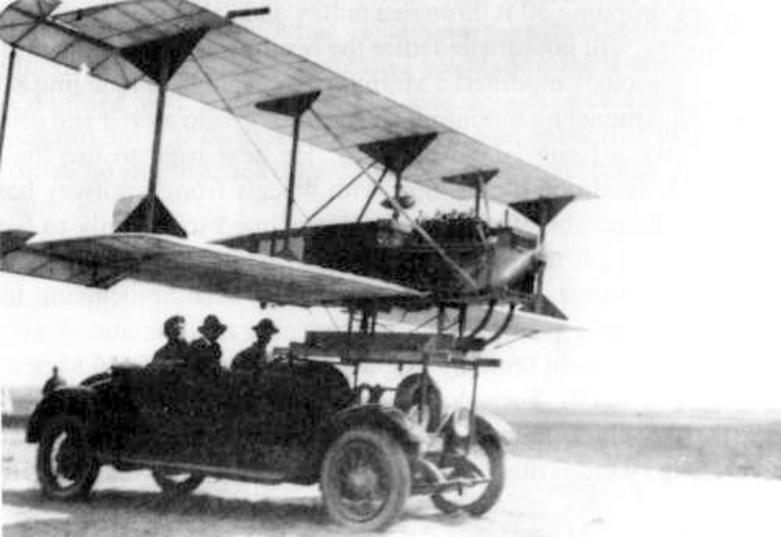
\includegraphics[width=0.8\textwidth]{/Hewitt-Sperry.jpg}
\caption[Torpedo aéreo de Sperry]{Torpedo aéreo de Sperry}
\label{fig:hewittsperry}
\end{center}
\end{figure}

Los primeros sistemas fueron creados como armamento de largo alcance en artefactos tales como el torpedo aéreo de Sperry, mencionado anteriormente, y el blanco aéreo británico Aerial Target. El Aerial Target era un monoplano, sin piloto, controlado por radio que sirvió para verificar la viabilidad de utilizar señales de radio como sistema de guiado.

En el transcurso de la \textbf{Segunda Guerra Mundial}, Gran Bretaña abandonó la elaboración de misiles de crucero y se introdujo en el sector de los blancos aéreos con control completo por radio, a pesar de que el alcance era muy limitado.
En paralelo en Estados Unidos se fabricó el RP-4 (ver Figura~\ref{fig:rp4}) de Radioplane Company. A través de estos aviones, se fue perfeccionando la tecnología y el uso del control remoto por radio (ver Figura~\ref{fig:controlador}).

\begin{figure}[!h]
\begin{center}
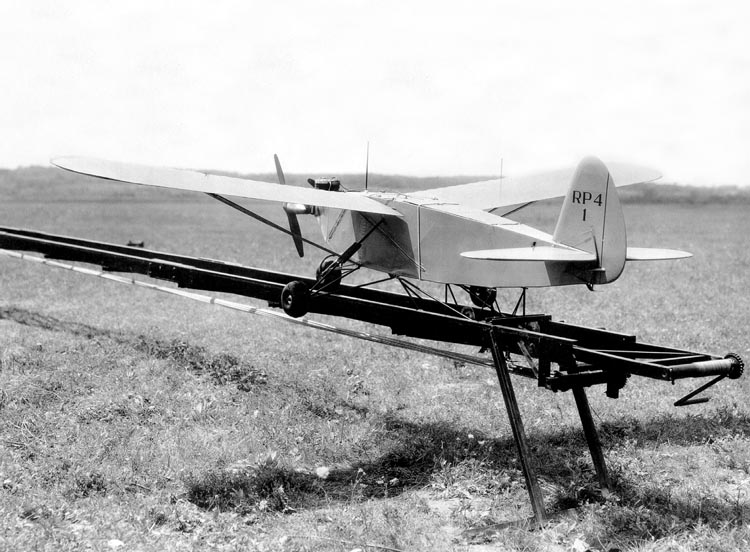
\includegraphics[width=0.8\textwidth]{/rp4.jpeg}
\caption[RP-4 listo para volar]{RP-4 listo para volar}
\label{fig:rp4}
\end{center}
\end{figure}


\begin{figure}[!h]
\begin{center}
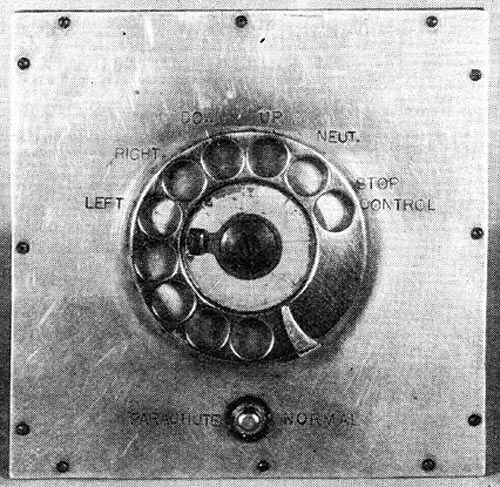
\includegraphics[width=0.65\textwidth]{/rp4controlador.jpeg}
\caption[Controlador de vuelo]{Controlador de vuelo}
\label{fig:controlador}
\end{center}
\end{figure}

En la \textbf{Posguerra} de la \textbf{Segunda Guerra Mundial}, la compañía Northrop produjo una serie de blancos aéreos no tripulados, llamados Falconer (ver Figura~\ref{fig:northrop}), que llevaban integrados sistemas de radiocontrol más modernos. 
Otra aplicación relevante durante la \textbf{Posguerra} fue la de señuelos antirradar (ver Figura~\ref{fig:northrop}). Estos eran soltados desde bombarderos, donde también eran controlados por radio con la ayuda de imágenes de vídeo, con la finalidad de confundir a los sistemas radar enemigos.

\begin{figure}[!h]
\begin{center}
\subfigure[Northrop Falconer]{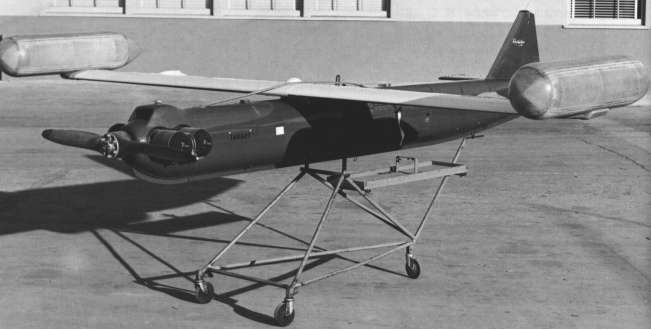
\includegraphics[width=0.6\textwidth]{/falconer.jpg}}
\subfigure[Señuelo antirradar Northrop Crossbow]{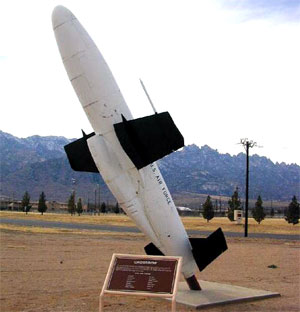
\includegraphics[width=0.3\textwidth]{/crossbow.jpg}}
\caption[Aeronaves no tripuladas de la compañia Northrop]{Aeronaves no tripuladas de la compañia Northrop}
\label{fig:northrop}
\end{center}
\end{figure}

Con la aparición de aviones militares con sistemas de propulsión a reacción, a lo largo de \textbf{1960}
se fabricaron blancos aéreos más rápidos y con mayor alcance (ver Figura~\ref{fig:ryanfirebee}). De esta manera, eran más difíciles de detectar y de derribar que los aviones de reconocimiento tripulados y, adicionalmente, no provocarían incidentes diplomáticos asociados con la captura de un piloto. 
Posteriormente estos \acs{UAV}s fueron equipados con cámaras para misiones de reconocimiento, revelando las fotos en la base cuando el \acs{UAV} regresaba. Algunos incluso incorporaron buscadores de radiación y cabezas de combate antirradar.

\begin{figure}[!h]
\begin{center}
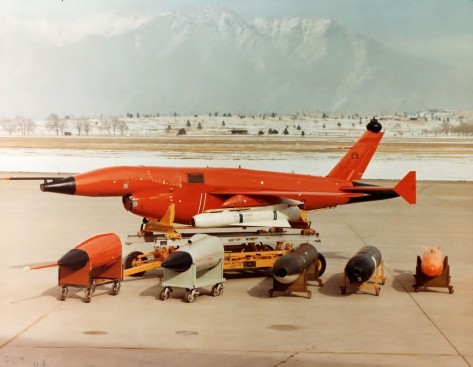
\includegraphics[width=0.8\textwidth]{/ryanfirebee.jpg}
\caption[Ryan Firebee]{Ryan Firebee}
\label{fig:ryanfirebee}
\end{center}
\end{figure}

Los \textbf{años 70} iban a ser testigos de la inclusión de \acs{UAS} en misiones de 
reconocimiento y vigilancia tanto de corto alcance, como de largo alcance y elevada altitud. Fueron sistemas 
más complejos tanto en los requisitos de la misión como en la seguridad en las comunicaciones.

En \textbf{1980} se creó un sistema en el que el \acs{UAV} se lanzaba desde una rampa (ver Figura~\ref{fig:cl89}) y se rescataba con un paracaídas y un airbag. 
Cuando se realizaban análisis diurnos el \acs{UAV} estaba equipado con una cámara convencional más una cámara de infrarrojos y para los análisis nocturnos únicamente se equipaba la cámara infrarroja. El guiado se llevaba a cabo mediante la preprogramación de un autopiloto basándose en giróscopos verticales y direccionales, información de altímetros y anemómetros barométricos. 
Además, transportaba un transmisor de video que podía enviar imágenes, en tiempo real, a la estación de control 
en tierra, estando a 70 km de la base.

\begin{figure}[!h]
\begin{center}
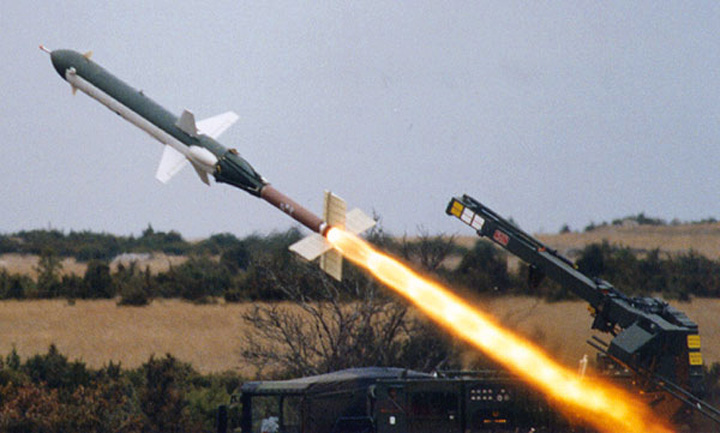
\includegraphics[width=0.8\textwidth]{/cl-289-09.jpg}
\caption[Lanzamiento del Canadair CL-89]{Lanzamiento del Canadair CL-89}
\label{fig:cl89}
\end{center}
\end{figure}

En los \textbf{años 90} con la mayor disponibilidad del \acs{GPS} y de las comunicaciones vía satélite se consigue que los \acs{UAS} puedan operar por encima de la señal de radio y que puedan abandonar el uso de sistemas de navegación imprecisos basados en giróscopos y
datos de aire. Es así como, junto con los sistemas digitales de control de vuelo o \acs{DFCS}, el alcance y la precisión de la navegación mejoraron apreciablemente. 
Como resultado se desarrollaron sistemas de medio y largo alcance. 

En la \textbf{década de los 2000} se produce un incremento en el uso militar de los sistemas no tripulados. 
Por otro lado, las posibles aplicaciones civiles no han fructificado debido a la dificultad a la hora de asegurar la 
separación entre las aeronaves tripuladas y no tripuladas.
Otro paso adelante en esta década fue la instalación de armamento en \acs{UAV}s para una respuesta inmediata ante el posible 
descubrimiento de fuerzas enemigas.
Otras líneas de avance, en este periodo de tiempo, son las que tratan de aumentar la automatización, reduciendo así
la carga de trabajo y los errores de las tripulaciones en tierra.

\textbf{Más allá del 2010}, el mercado militar de los \acs{RPAS} continúa con una tendencia positiva desde el final de la Guerra Fría y se espera que se acelere en las primeras décadas del siglo XXI. La tendencia comercial en el mercado de la robótica está también en constante crecimiento (ver Figura~\ref{fig:prevision}). Como consecuencia de esta corriente, la tecnología está apoyando estas tendencias con microprocesadores cada vez más baratos y competentes que incentiven su utilización.

\begin{figure}[!h]
\begin{center}
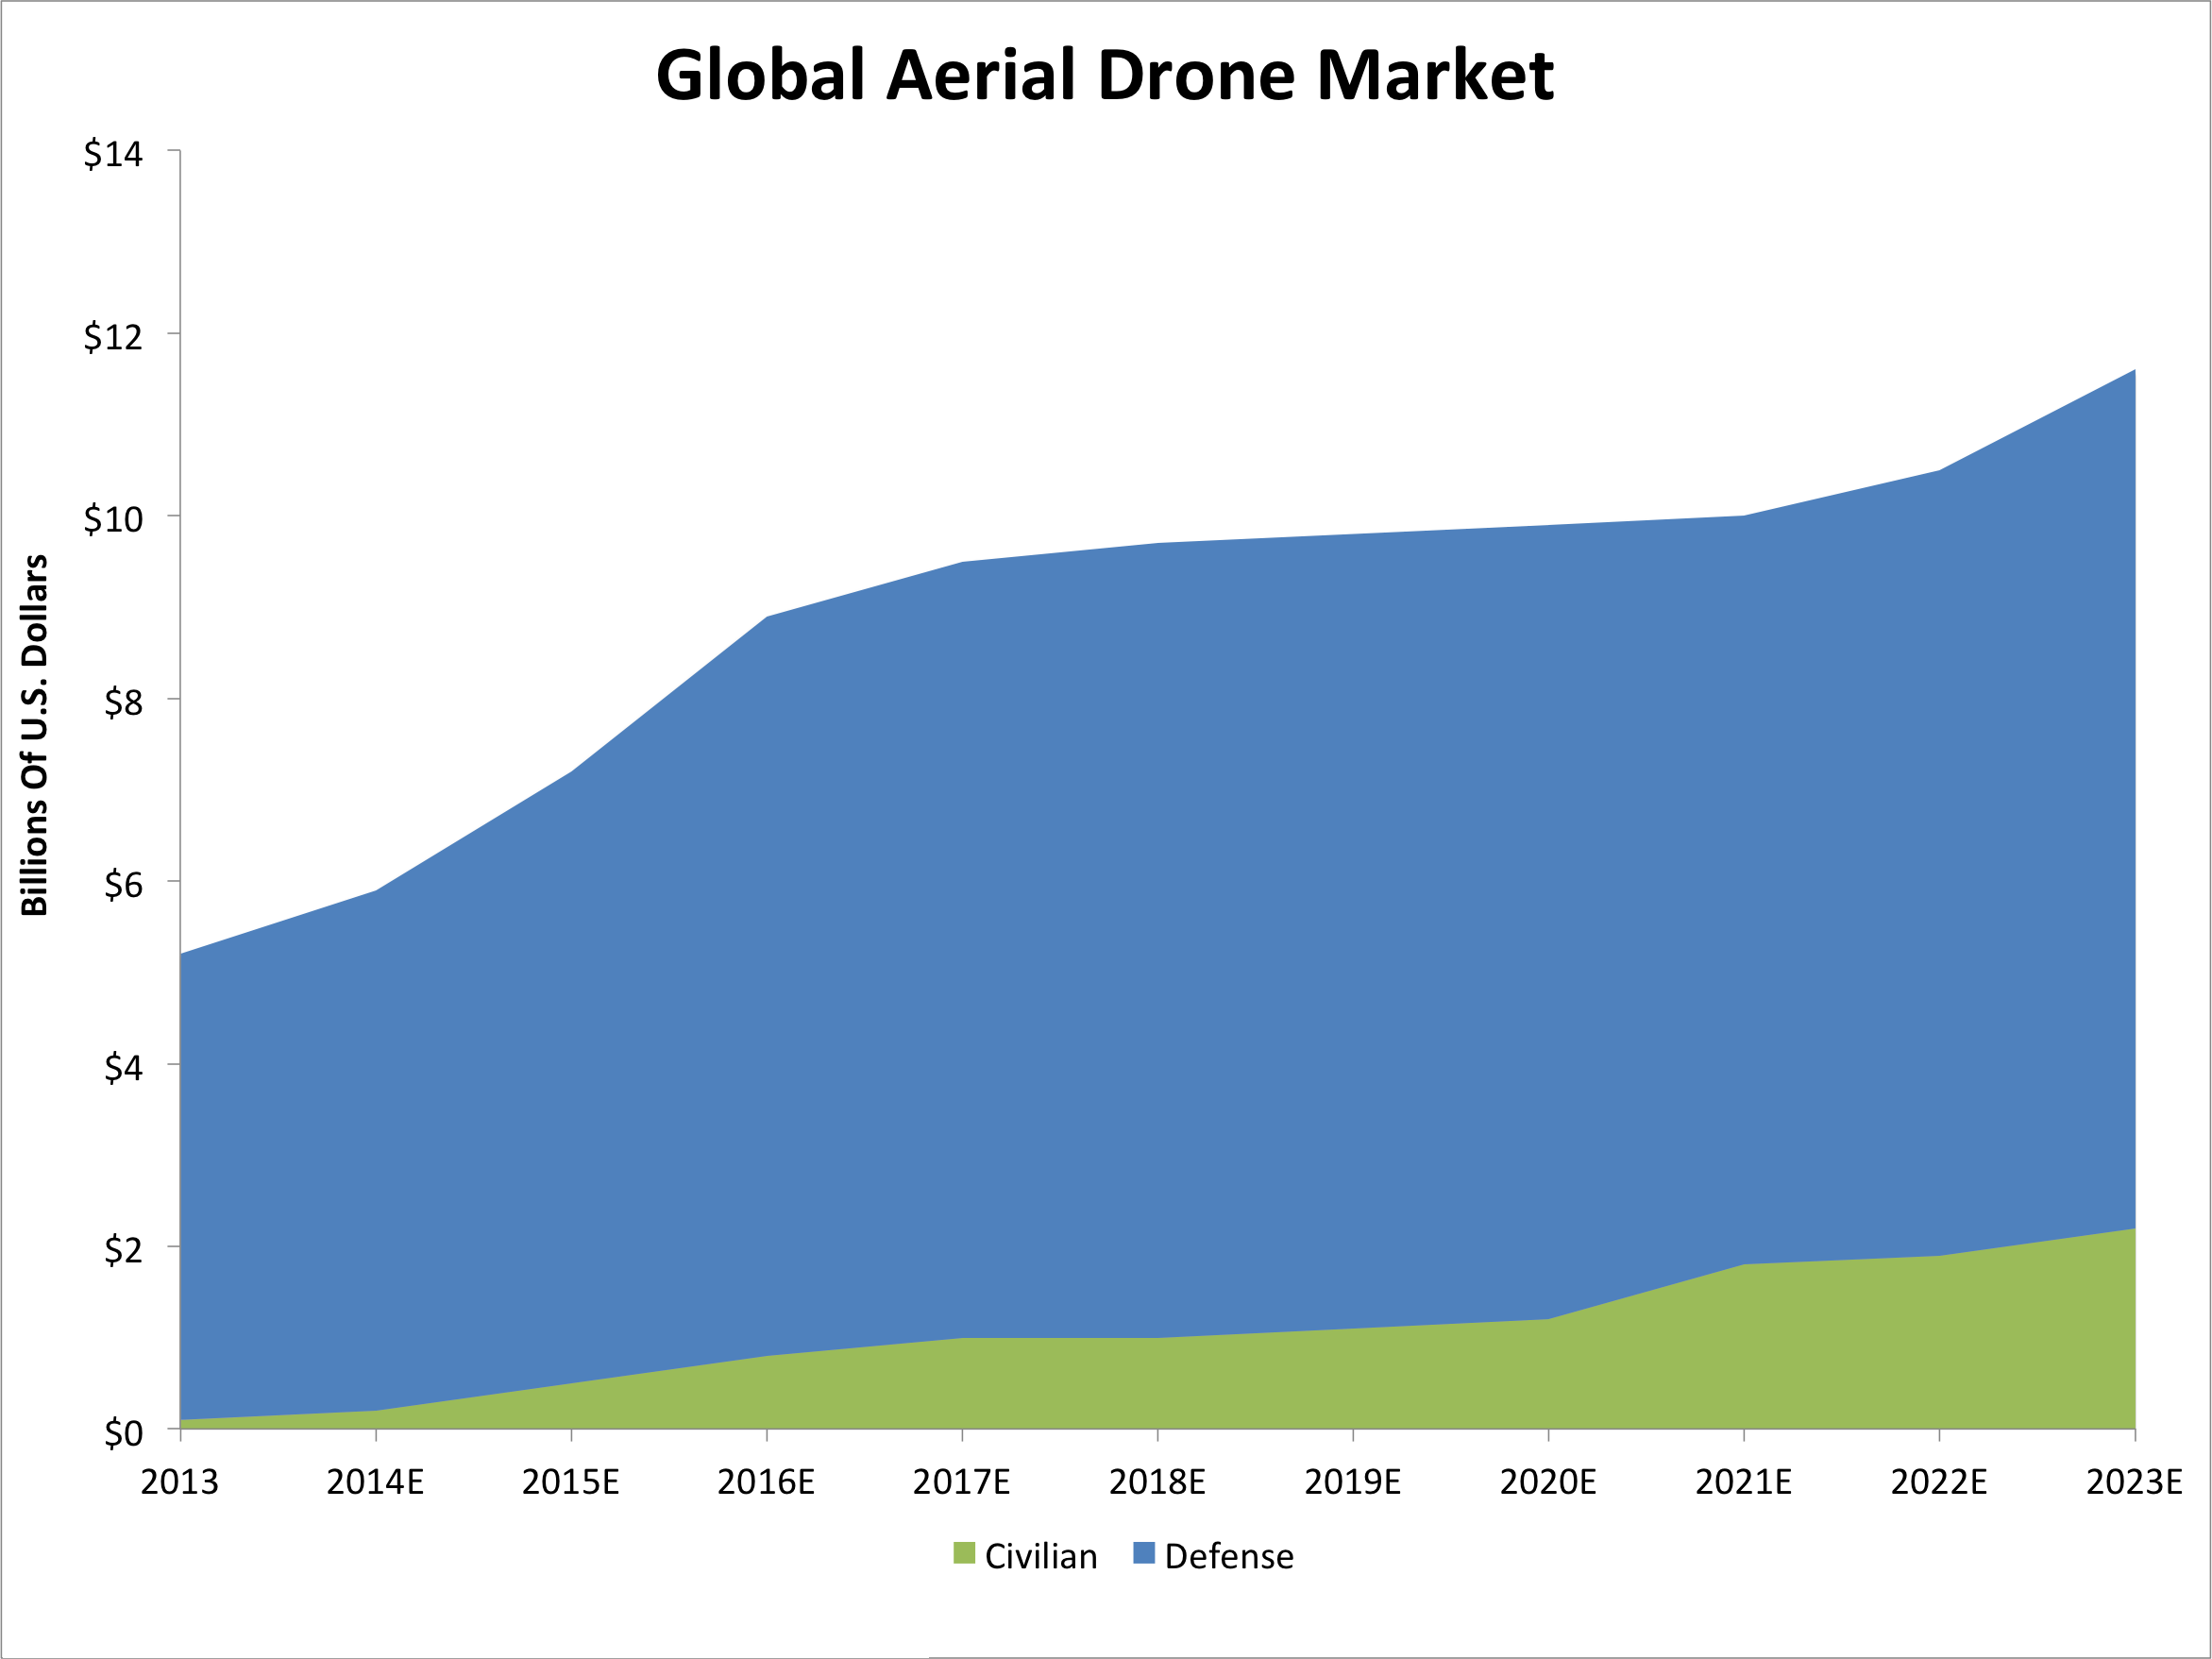
\includegraphics[width=0.8\textwidth]{/prevision.png}
\caption[Estimación del mercado de drones en el periodo 2013-2023]{Estimación del mercado de drones en el periodo 2013-2023 \cite{prevision}}
\label{fig:prevision}
\end{center}
\end{figure}

\subsection{Tipos de aeronaves pilotadas por control remoto}
\label{sec:tipos}

En conformidad con la Organización de Aviación Civil Internacional, «El hecho de que la aeronave sea tripulada o no tripulada no afecta su condición de aeronave. Cada categoría de aeronave tendrá posiblemente versiones no tripuladas en el futuro.
Este punto es fundamental para todos los aspectos futuros relativos a las \acs{UA} y proporciona la base para tratar la aeronavegabilidad, el otorgamiento de licencias al personal, las normas de separación, etc.» \cite{OACI}. En otras palabras, las aeronaves no tripuladas son, en primer lugar, aeronaves, por lo que están sujetas a las mismas normas y restricciones que las aeronaves tripuladas.

Existen múltiples formas de clasificar las aeronaves, pero lo habitual es utilizar una clasificación atendiendo al modo en la que las aeronaves consiguen su sustentación en la atmósfera. A continuación se propone una clasificación en la que se presenta los principales tipos de aeronaves:  

\begin{itemize}
\item \textbf{Aerostato}: Más ligeros que el aire.
	\begin{itemize}
	\item Globo aerostático.
	\item Dirigible.
	\end{itemize}
\item \textbf{Aerodino}: Más pesados que el aire.
	\begin{itemize}
	\item \textbf{Ala fija}.
		\begin{itemize}
		\item Avión.
		\item Planeador.
		\item Ala delta.
		\item Parapente.
		\item Paramotor.
		\end{itemize}
	\item \textbf{Ala rotatoria}.
		\begin{itemize}
		\item Helicóptero.
		\item Multirrotor.
		\item Autogiro.
		\end{itemize}
	\end{itemize}
\end{itemize}

Por otra parte, aparecen aeronaves de nuevas clases, como los híbridos, que ejecutan parte del vuelo haciendo uso del método de ala rotatoria, generalmente en el despegue y aterrizaje, realizando un salto al uso de ala fija para dirigirse de forma rápida y eficiente a su destino.

El uso de vehículos aéreos no tripulados ha alcanzado un grado de madurez significativo en el terreno militar. Tanto es así, que 
en el ejército norteamericano constituyen cerca de un tercio de la flota de aeronaves, desempeñando en exclusiva las misiones 
de inteligencia, vigilancia y reconocimiento que deben cumplir las fuerzas armadas. «De acuerdo con la consultora de defensa Teal Group Corporation \footnote{\url{http://www.tealgroup.com}}, el inventario en 2013 de sistemas aéreos no tripulados contaba con más de 10.000 \acs{UAS} (ver Figura~\ref{fig:flota})  [...], de lo que se deduce que en el ámbito militar la preponderancia de los sistemas de ala fija (ver Figura~\ref{fig:alafija}) es casi absoluta (97\%)» \cite{dron2}.

\begin{figure}[!h]
\begin{center}
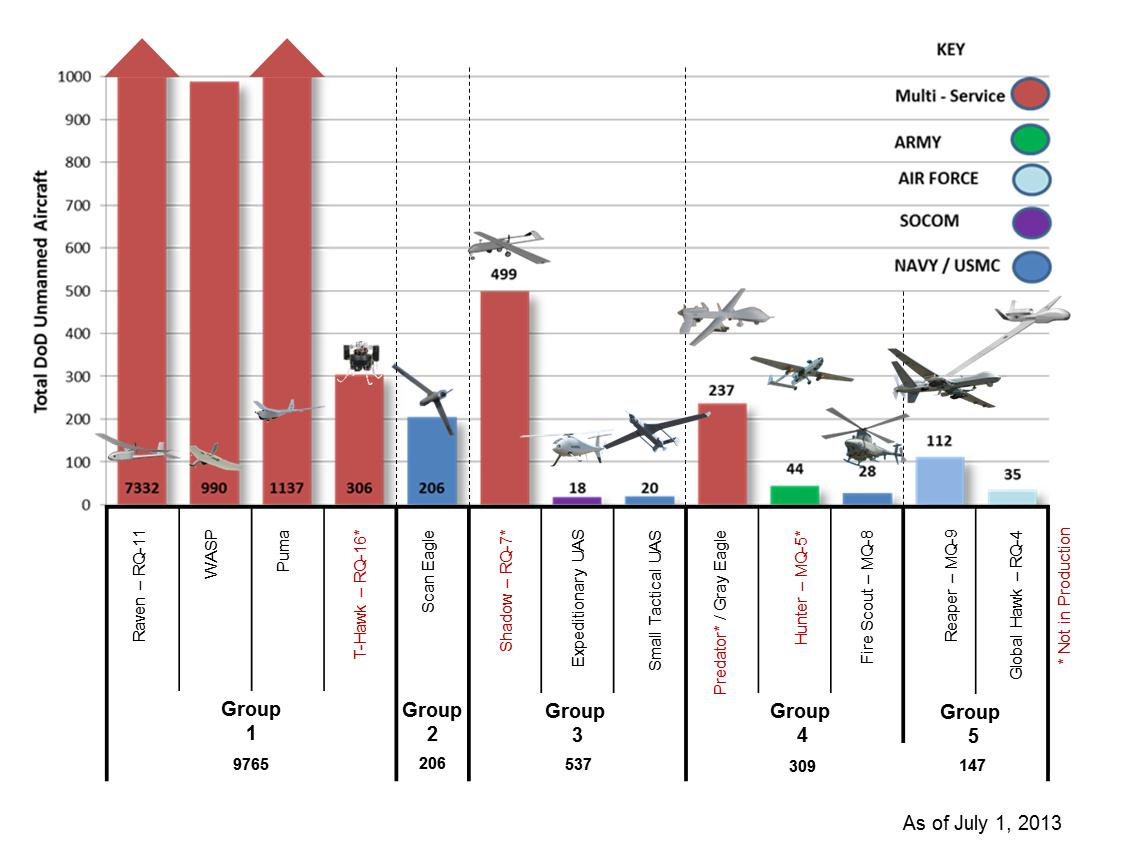
\includegraphics[width=0.8\textwidth]{/flota.jpg}
\caption[Aviones no tripulados del Departamento de Defensa de EE.UU. en el 2013]{Aviones no tripulados del Departamento de Defensa de EE.UU. en el 2013 \cite{ambitocivil2}}
\label{fig:flota}
\end{center}
\end{figure}


\begin{figure}[!h]
\begin{center}
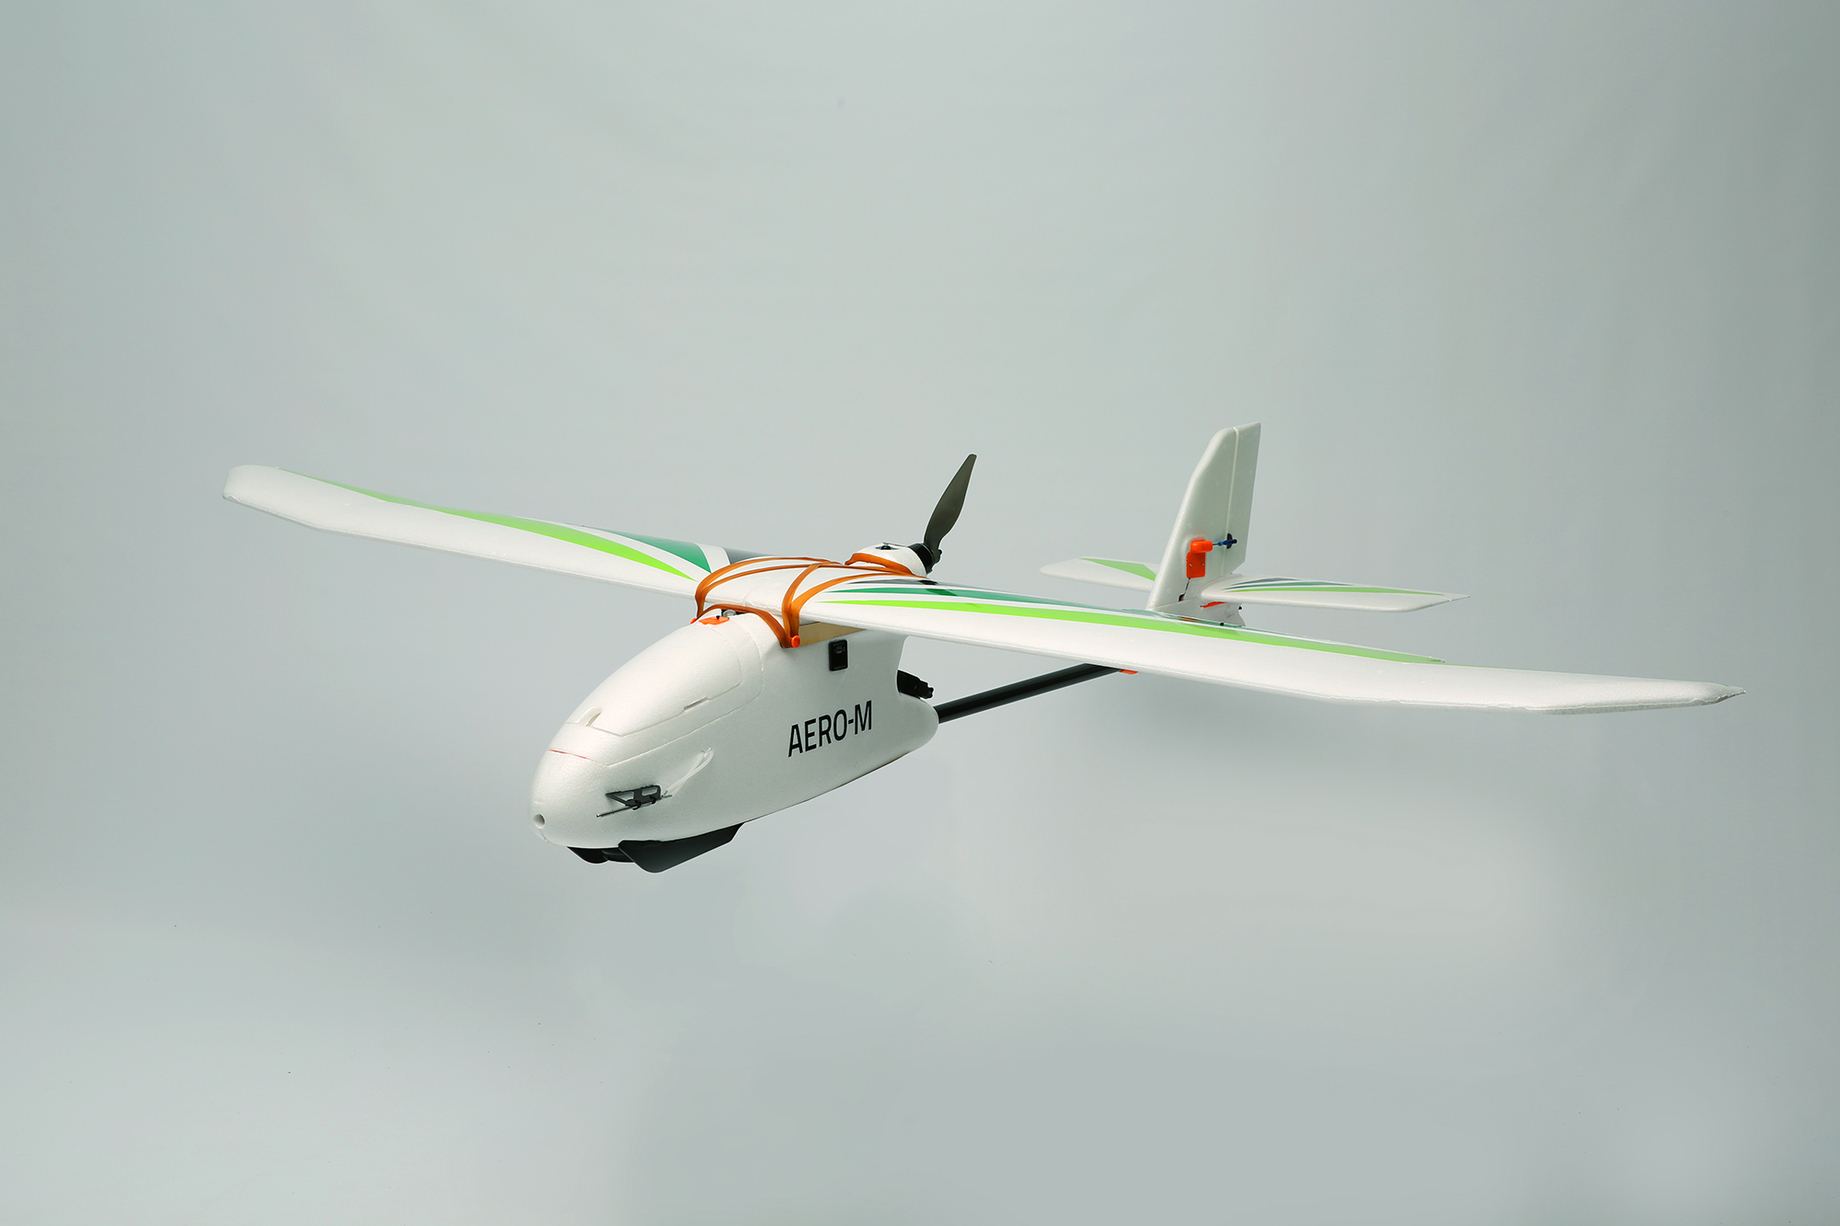
\includegraphics[width=0.8\textwidth]{/alafija.jpg}
\caption[Sistema de ala fija]{Sistema de ala fija}
\label{fig:alafija}
\end{center}
\end{figure}

En el ámbito civil, mucho menos avanzado que el militar, la situación es la contraria. «De acuerdo con la información suministrada por la Dirección General de la Aviación Civil francesa \footnote{\url{http://www.developpement-durable.gouv.fr/-Secteur-Aerien,1633-.html}} (DGAC) referida a las autorizaciones otorgadas hasta octubre de 2013, [...] los sistemas basados en aeronaves de ala rotatoria superan ampliamente
a los de otros tipos, si bien no de forma tan aplastante como ocurre en el mundo militar, ya que sólo suponen un 76\% del total» \cite{dron2}.

Esta inclinación, hacia las aeronaves multirrotor (ver Figura~\ref{fig:multirrotor}) en el entorno civil, se debe a que son altamente apropiadas para la principal actividad desempeñada en estos momentos, la toma de imágenes y videos, que según las estimaciones de la Asociación Española de RPAS \footnote{\url{http://www.aerpas.es/}} constituyen posiblemente más del 90\% de las tareas ejecutadas por drones \cite{AERPAS}, al igual que ocurre en otros países europeos.

\begin{figure}[!h]
\begin{center}
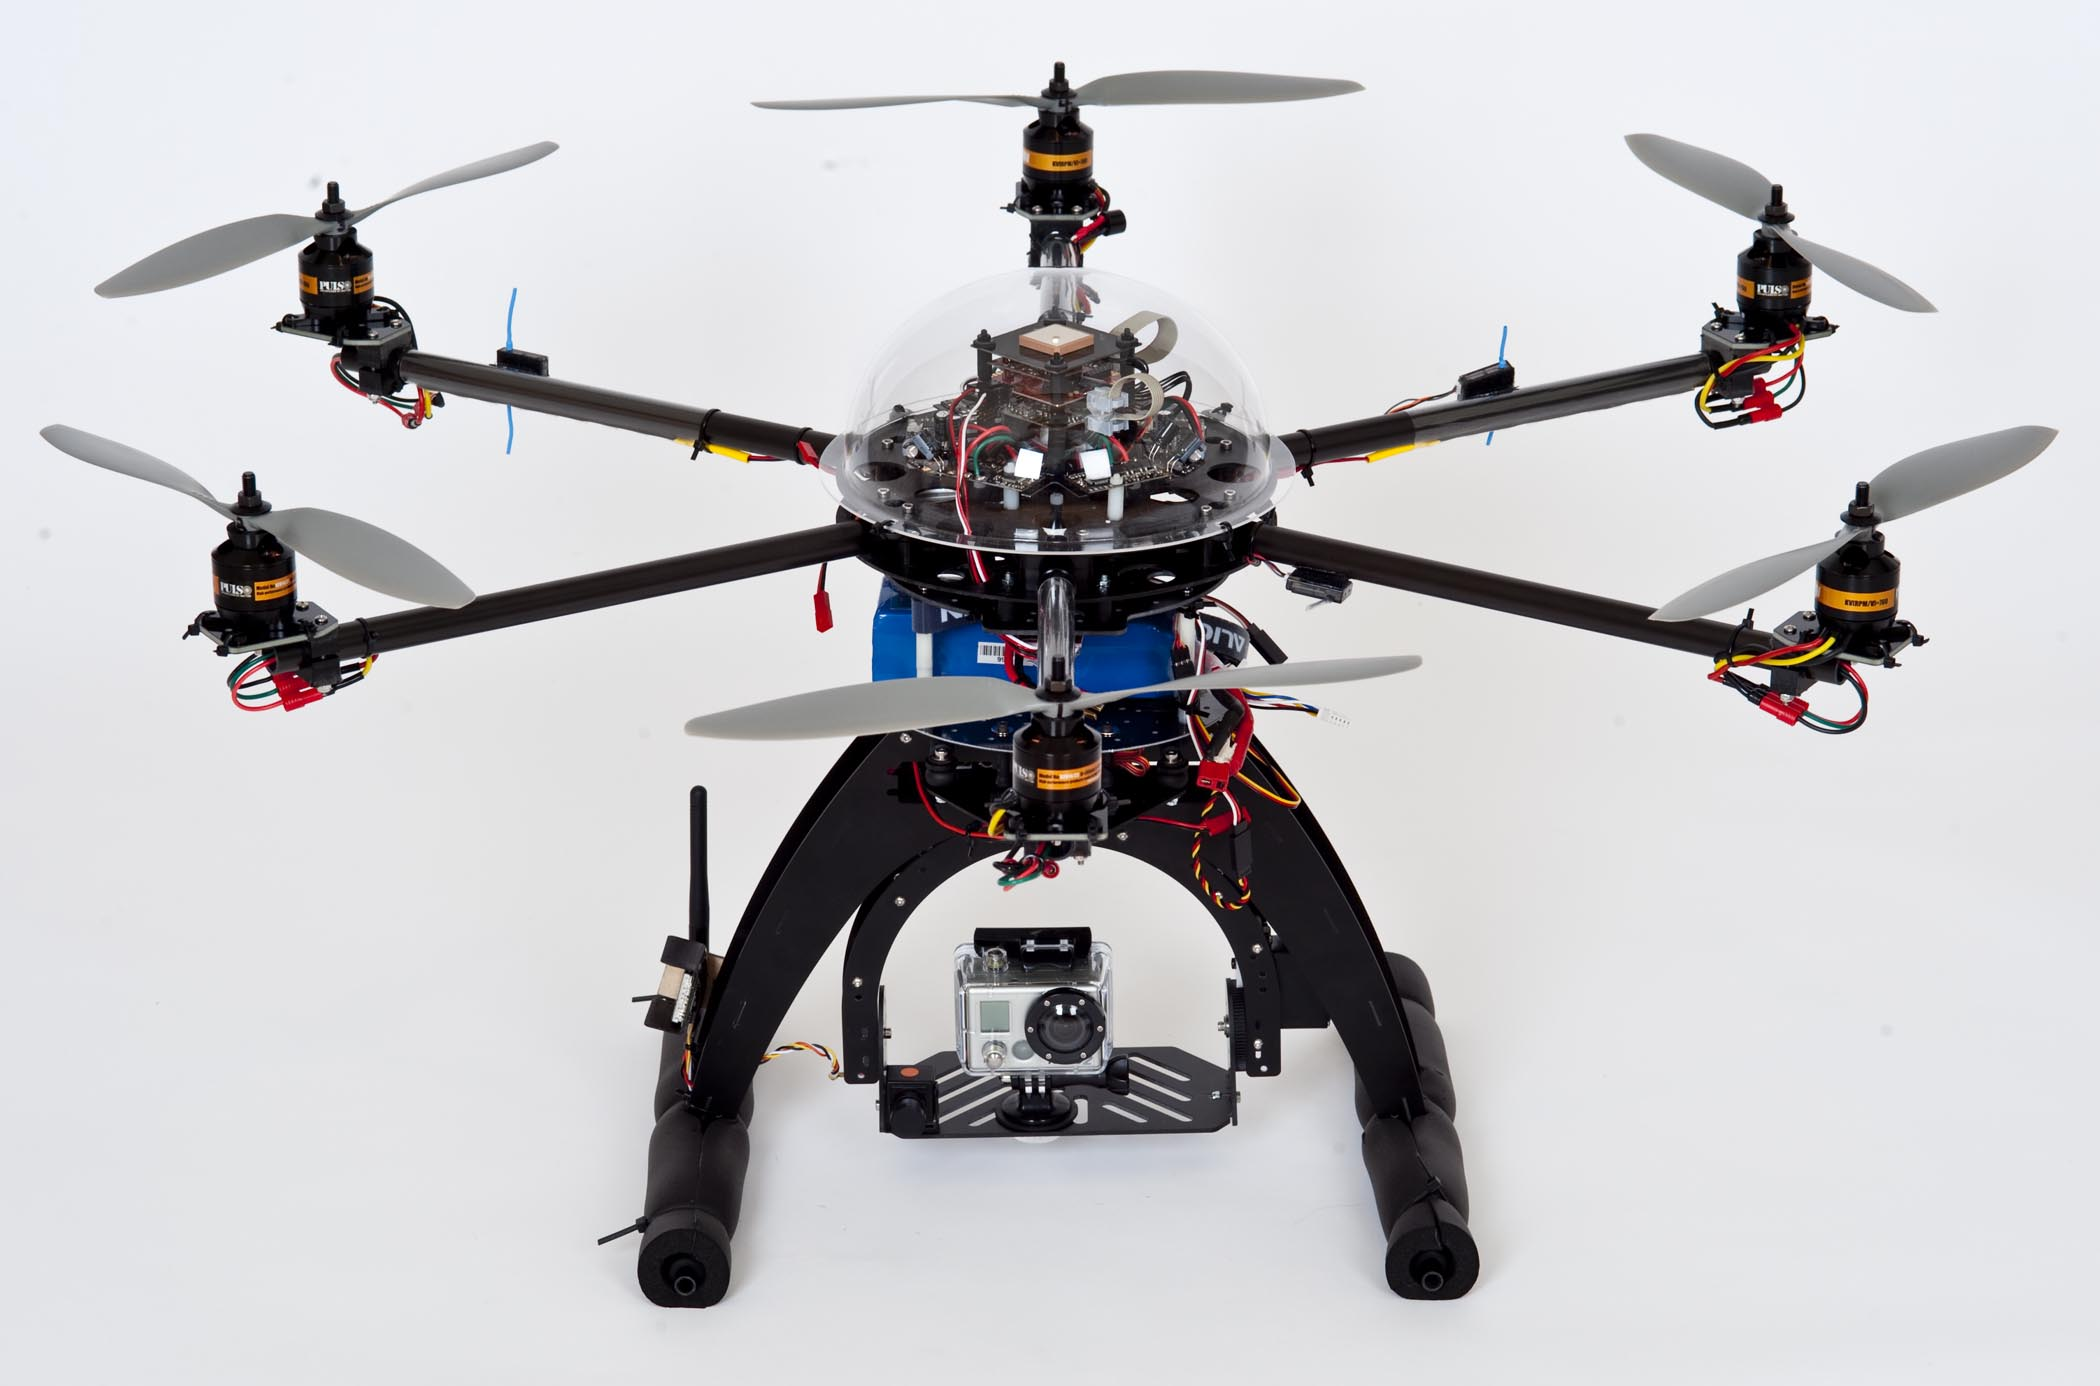
\includegraphics[width=0.8\textwidth]{/multicopter.jpg}
\caption[Sistema multirrotor]{Sistema multirrotor}
\label{fig:multirrotor}
\end{center}
\end{figure}

Las principales ventajas de los multirrotores son las siguientes:

\begin{itemize}
\item \textbf{Despegue y aterrizaje vertical}: que minimiza las necesidades del espacio requerido en tierra para su puesta en marcha	.
\item La posibilidad de \textbf{volar a punto fijo} o \textbf{a muy baja velocidad}: lo cual resulta idóneo para software en la que la observación sea un requisito vital.
\item Mayor \textbf{maniobrabilidad} y \textbf{precisión} de vuelo: mientras que los sistemas de ala fija siguen rutas curvilíneas, los multirrotores son capaces de volar siguiendo cualquier trayectoria deseada en las tres dimensiones.
\item Su diseño les permite acarrear \textbf{cargas más voluminosas}, en relación con su propio tamaño, que los aviones.
\end{itemize}

Por el contrario, los multirrotores tienen una serie de desventajas frente a los sistemas de ala fija:

\begin{itemize}
\item Son \textbf{menos eficientes}: lo que provoca que aunque tenga el mismo tamaño, la autonomía sea menor.
\item Vuelan a \textbf{menor velocidad}: lo que combinado con su menor autonomía significa que pueden cubrir un área mucho menor.
\item Tienen una \textbf{huella sonora sensiblemente mayor}, por lo que resultan poco indicados para operaciones de vigilancia.
\end{itemize}

A la vista de lo expuesto anteriormente se justifica que los multirrotores dominen hoy en día el mercado, 
«si bien es previsible que en el futuro, a medida que se desarrollen aplicaciones de ejecución más complejas, cubriendo 
mayores distancias y desarrolladas a mayor altura sobre el terreno, al igual que ocurre en el caso militar, los sistemas de ala 
fija aumentarán su peso» \cite{dron2}.

\subsection{Modos de operación en el guiado de una aeronave no tripulada}
\label{sec:mododeoperacion}

Sólo existen cuatro modos de operación en cuanto a la manera de guiar una aeronave de forma remota, 
con un grado de automatización creciente:

\begin{itemize}
\item \textbf{Modo manual}: el piloto remoto actúa sobre las superficies de control y la potencia de los motores, 
a través de una emisora de radiocontrol.
\item \textbf{Modo asistido}: similar al modo manual, pero el piloto remoto no interviene directamente sobre las superficies de 
control o los motores, sino que indica sus intenciones (girar a la derecha, subir, etc.), desde el puesto de radiocontrol, y el 
autopiloto las transforma en actuaciones que logren ese propósito.
\item \textbf{Modo automático}: el piloto remoto traza un plan de vuelo, es decir, un número de puntos de paso o «waypoints» antes del 
inicio del vuelo. La aeronave dispone de un piloto automático que sigue el plan previsto, realizando automáticamente las acciones 
requeridas en cada momento. Aun así el piloto mantiene el control en todo momento, pudiendo modificar los puntos de paso durante el vuelo, ejecutar maniobras predeterminadas (como por ejemplo la «vuelta a casa») o incluso tomar el control directamente.
\item \textbf{Modo autónomo}: es semejante al modo automático, en cuanto que se establece un plan de vuelo con anterioridad, 
pero una vez iniciado el vuelo se continúa con el plan de forma completamente autónoma, sin precisar la intervención del piloto 
incluso en caso de producirse situaciones de emergencia.
\end{itemize}

Es obvio que el modo manual y el modo asistido requieren que la aeronave se encuentre a la vista del piloto o, que al menos, 
transmita información suficiente para que el piloto posea el conocimiento necesario de la situación y del escenario como para poder tomar las decisiones adecuadas. Por ello, el uso de estos modos suele estar restringido a las circunstancias de vuelo en línea de vista visual o \acs{VLOS}.

Se destaca el hecho de que el modo manual se utiliza normalmente en las aeronaves de ala fija. Las de ala rotatoria, 
sobre todo los multirrotores, suelen utilizar el modo asistido, por la dificultad que implica el coordinar todas las acciones 
para mantener la aeronave estabilizada y ejecutar las maniobras deseadas. En ambos casos es necesaria una considerable destreza 
por parte del piloto para controlar la aeronave desde tierra.

Por esta razón existe una tendencia a utilizar de forma exclusiva \acs{RPAS} en modo automático, o por lo menos en una forma de modo 
asistido en la que el piloto recibe una imagen tomada por una cámara dirigida hacia adelante, denominada visión en primera persona 
o \acs{FPV}, lo que le permite actuar como si estuviera embarcado en ella. Este modo resulta también muy indicado en vuelos en línea de vista para misiones rutinarias. La principal ventaja que proporciona el modo automático es la posibilidad de utilizar pilotos de menor capacitación y, por lo tanto, de reducir el coste de operación.

\subsection{Visión por computador en \acs{UAV}s}
\label{sec:visionporcomputador}

«La \textbf{visión por computador} es un campo de la inteligencia artificial en el que se busca, a través de lenguajes de programación, que un computador sea capaz de identificar y ejecutar órdenes con el reconocimiento de ciertas características de imágenes, imágenes completas o secuencias de éstas» \cite{visionporcomputador}.

Los sistemas de visión artificial están formados por: 
\begin{itemize}
\item Una \textbf{fuente de luz}.
\item Un \textbf{sensor de imagen} que capture las imágenes que después se procesan.
\item Una \textbf{tarjeta de adquisición de imágenes}, como interfaz entre sensor y el computador.
\item Una serie de \textbf{algoritmos de análisis} en los que se procesan, segmentan y se aplican las transformaciones necesarias para obtener los resultados deseados. 
\item Un \textbf{procesador} que analice las imágenes recibidas ejecutando los algoritmos diseñados. 
\item Un \textbf{sistema de respuesta} a tiempo real que ejecute los comandos.
\end{itemize}

El ser humano percibe la luz gracias a los ojos y la información captada se traslada al cerebro por el nervio óptico. El cerebro procesa la imagen, analiza la escena y actúa en consecuencia. Los sistemas de visión por computador buscan imitar este comportamiento, para lo cual, se definen cuatro fases (ver Figura~\ref{fig:fasescv}), estas fases son:

\begin{itemize}
\item \textbf{Captura}: se adquieren las imágenes.
\item \textbf{Procesamiento}: se aplican filtros o transformaciones que eliminan partes no deseadas, facilitando las próximas etapas.
\item \textbf{Segmentación}: se abstraen los elementos que interesan del resto de la imagen para su comprensión.
\item \textbf{Reconocimiento}: se distinguen los objetos segmentados haciéndose uso de una serie de características que previamente se han establecido.
\end{itemize}

\begin{figure}[!h]
\begin{center}
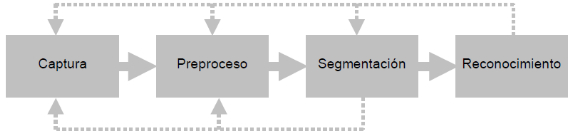
\includegraphics[width=0.8\textwidth]{/fasescv.jpg}
\caption[Fases de un sistema de visión por computador]{Fases de un sistema de visión por computador \cite{visionporcomputador}}
\label{fig:fasescv}
\end{center}
\end{figure}

En el campo de los sistemas aéreos no tripulados, la visión por computador es una parte importante para la navegación y el control, 
y en ella se basan numerosas aplicaciones. Los \acs{UAV}s aparecen como una alternativa barata y adecuada en muchas campos
de aplicación, dadas sus capacidades de vuelo y a la posibilidad de integrar sistemas de visión que permiten mejorar determinadas 
tareas como el pilotaje, el guiado autónomo del vehículo o la obtención de imágenes.

En la actualidad, se han desarrollado aplicaciones con vehículos aéreos no tripulados, que hacen uso de la visión por computador, en distintos ámbitos de aplicación como: la gestión del tráfico \cite{controltrafico}, la detección de incendios \cite{incendios} o la evitación de obstáculos \cite{obstaculos}.

\subsection{Aplicación de \acs{UAV}s en el sector civil}
\label{sec:ingenieriacivil}

Los drones pueden ser calificados como robots no antropomorfos con una enorme autonomía de vuelo y con un abanico de posibilidades de  aplicación.

«Gracias al uso de procesadores electrónicos, de software especializado y del Sistema de Posicionamiento Global (\acs{GPS}), las capacidades de control automático en base a la información procedente de los sensores instalados en las aeronaves, y la rápida reacción correctiva como consecuencia del procesamiento local de la información del estado de vuelo, hacen posible que la retroalimentación aporte un inmenso potencial,
minimizando para estos artefactos las posibles desviaciones entre el comportamiento real y el esperado» \cite{ambitocivil}.

Actualmente, haciendo caso omiso a los usos bélicos, estos equipos brindan \textbf{amplias oportunidades} de aplicación \textbf{al sector de la ingeniería civil} (ver Cuadro~\ref{tab:ambitocivil2}): investigación atmosférica, filmación de películas y fotografía deportiva, gestión de riegos y desastres naturales, inspecciones de infraestructuras, levantamientos topográficos, agricultura de precisión, control de caza, localización de bancos de pesca, mantenimiento de parque eólicos e infraestructuras energéticas (ver Figura~\ref{fig:unionfenosa}), control medioambiental, exploración geológico-minera, etc.

\begin{figure}[!h]
\begin{center}
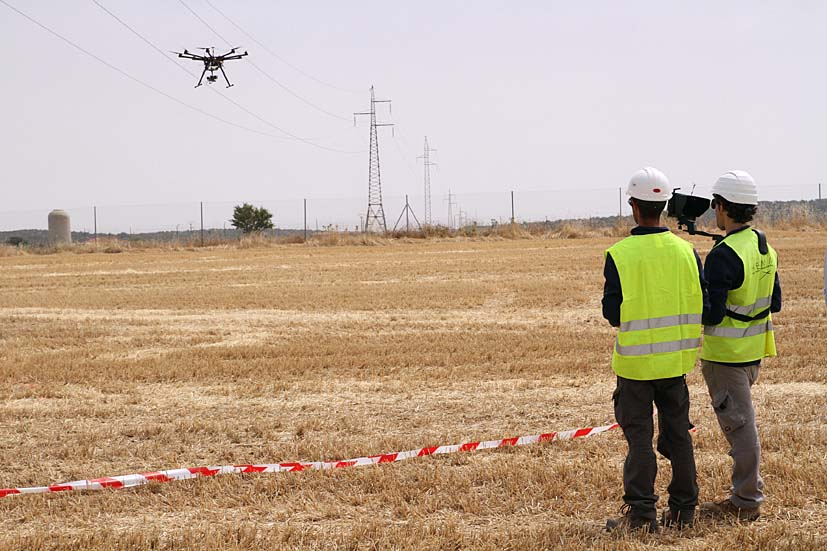
\includegraphics[width=0.8\textwidth]{/drones-6.jpg}
\caption[Revisión de líneas eléctricas con drones en Ciudad Real]{Revisión de líneas eléctricas con drones en Ciudad Real \cite{unionfenosa}}
\label{fig:unionfenosa}
\end{center}
\end{figure}


\begin{table}[htbp]
  \centering
  {\small
  \begin{tabular}{p{.17\textwidth}p{.15\textwidth}p{.15\textwidth}p{.15\textwidth}p{.15\textwidth}}
  \tabheadformat
  \tabhead{Fecha} &
  \tabhead{Actividad} &
  \tabhead{Lugar} &
  \tabhead{Usuario}  &
  \tabhead{Operador}	\\
\hline
Enero 2014  & Cartografía & Suiza & Pix4D & ATyges \\

\hline
Enero 2014  & Vigilancia de fronteras & California & Homeland Security Department & \\
    
\hline
Enero 2014  & Formación & Madrid &  & CB Group Universidad Politécnica \\  

\hline
Enero 2014  & Protección Civil & Extremadura & Junta de Extremadura  & ATyges \\

\hline
Enero 2014  & Experimentación y ensayos & Villacarrillo & Centro ATLAS  & Boeing \\

\hline
Diciembre 2013  & Seguridad ciudadana & Madrid & Ayuntamiento de Madrid  & Policía Local \\
  
\hline
Diciembre 2013  & Entrega de paquetería & EE.UU. & Amazon & Amazon Prime Air \\

\hline
Noviembre 2013  & Apoyo a ciclo de vida & Francia & Ejército de Tierra & ADS \\          

\hline
Noviembre 2013  & Revisión de infraestructura & Viaducto de Roquemaure & SNCF Francia & Diades, Red Bird, Azur Drones \\

\hline
Noviembre 2013  & Pruebas de vuelo e infraestructura & Villacarrillo & Centro ATLAS & FADA - CATEC \\ 

\hline
Octubre 2013  & Inspección de cultivos & Jerez de la Frontera & Proyecto Fieldcopter & \\

\hline
Octubre 2013  & Prevención de incendios &  & Junta de Andalucía & ELIMCO \\

\hline
Octubre 2013  & Asistencia sanitaria & Alemania & Definetz &  \\

\hline
Septiembre 2013  & Publicidad & Madrid & Candidatura Madrid 2020 &  \\

\hline
Septiembre 2013  & Lucha contra incendios & California & Guardia Nacional & Guardia Nacional  \\

\hline
Septiembre 2013  & Investigación medioambiental & Antártida & NASA & Universidad de Colorado  \\

\hline
\end{tabular}


% Local variables:
%   coding: utf-8
%   ispell-local-dictionary: "castellano8"
%   TeX-master: "main.tex"
% End:

  }
  \caption[Principales actividades civiles desde septiembre de 2013]
  {Principales actividades civiles desde septiembre de 2013 \cite{ambitocivil2}}
  \label{tab:ambitocivil2}
\end{table}

En los países más avanzados se está fomentando el uso de estos aparatos en diferentes proyectos de investigación \cite{UA}, que abarcan desde el ensayo de material aeronáutico en condiciones peligrosas, pasando por el reparto de cargas, hasta el desarrollo de tecnologías, como las pilas de combustible de hidrógeno, que triplicarían la duración de los vuelos.

\section{Inteligencia Artificial Distribuida}
\label{sec:inteligenciaartificial}

La evolución de los procesadores multinúcleo y de las redes informáticas combinadas con que muchas actividades, incluyendo la resolución de problemas de las personas, involucran a grupos de gente condujo al desarrollo de un nuevo campo de investigación: la \textbf{Inteligencia Artificial Distribuida} (\acs{IAD}). Fusiona la Inteligencia Artificial (\acs{IA}) con la Computación Distribuida y es definida como «un subcampo de la \acs{IA} que se centra en los comportamientos inteligentes colectivos que son producto de la cooperación de diversas entidades» \cite{IAD}.

La \acs{IAD} aparece en la década de los 80 para estudiar los sistemas inteligentes, que están formados por un conjunto de varios agentes, e intenta resolver problemas donde una conducta colectiva es más eficiente que una conducta individual. Según Iglesias \cite{IAD2}, a pesar de ser una disciplina joven, podemos distinguir tres periodos cronológicos bien diferenciados:

\begin{itemize}
\item \textbf{\acs{IAD} clásica}: centrada en el estudio de la conducta colectiva, en oposición a la \acs{IA}, que estudia la conducta individual.
\item \textbf{\acs{IAD} autónoma}: focalizada en el estudio de los agentes individuales situados en un mundo social.
\item \textbf{\acs{IAD} comercial}: centrada en la aplicación de la \acs{IAD} clásica y autónoma, desarrollando agentes con características muy
diferenciadas que están siendo explotados de forma comercial.
\end{itemize}

El campo de investigación de la \acs{IAD} desencadenó en campos más específicos: la Inteligencia Artificial Paralela, la Resolución Distribuida de Problemas y los \textbf{Sistemas Multiagente} (\acs{SMA}). El nacimiento de estos \acs{SMA} implicó la irrupción de un nuevo paradigma en el desarrollo del software que no solo afectó en las fases de conceptualización, diseño e implementación, sino también en la aplicabilidad de las soluciones propuestas.  

\subsection{Sistemas Multiagente}
\label{sec:sismultiagente}

Cada agente «es un sistema computacional que está situado en algún entorno, y que es capaz de actuar autónomamente en dicho entorno con el fin de cumplir sus objetivos» \cite{agente}. Sin embargo, muchas aplicaciones requieren la interacción entre diversos individuos para poder alcanzar un determinado objetivo. Estos sistemas, compuestos de varios agentes, son denominados \textbf{Sistemas Multiagente}.

Un \acs{SMA} puede ser definido formalmente como «una organización o sociedad de agentes, donde un conjunto de agentes interactúan y cooperan entre sí para alcanzar algún objetivo colectivo» \cite{sma}.

De acuerdo con Sycara \cite{sma2}, un \acs{SMA} está caracterizado por lo siguiente:
\begin{itemize}
\item Cada agente tiene \textbf{información incompleta} o \textbf{no tiene} la \textbf{suficiente capacidad} para resolver el problema global. Es decir, tiene un punto de vista limitado.
\item \textbf{Necesitan} de formas de \textbf{coordinarse} .
\item Los \textbf{datos} están \textbf{descentralizados}.
\item Los \textbf{cálculos} son \textbf{asíncronos}.
\end{itemize}
 
La teoría de agentes y \acs{SMA} propicia dar un mayor realismo a la gestión de ciertos problemas, sumando a los modelos características que normalmente no se tienen en cuenta por la dificultad que incrementan al proceso de resolución del mismo. Cuando los problemas que se quieren solventar incorporan peculiaridades como: gran tamaño, alto grado de incertidumbre, dinamismo, o singularidad en la distribución de sus elementos, son extraordinarios candidatos a la aplicación de agentes para obtener ventajas en el proceso de resolución. 

Para que un \acs{SMA} pueda adaptarser rapidamente a los cambios de su entorno, los agentes deben poder \textbf{coordinarse} cuando es necesario realizar cambios en sus metas o en los roles que tienen asignados.

\subsection{Esquemas de coordinación}
\label{sec:esquemascoordinacion}

La comunicación adquiere relevancia en el comportamiento de los agentes en el momento de coordinar sus acciones, consiguiendo sistemas más consistentes. 

«La \textbf{coordinación} es una propiedad de los \acs{SMA} que posibilita el desarrollo de una acción en un entorno compartido. El grado de coordinación determinará hasta que punto el sistema es capaz de evitar acciones innecesarias o ajenas para minimizar el gasto de recursos, evitar situaciones de bloqueo y mantener unas determinadas condiciones de seguridad» \cite{coordinacion}. Ejemplos convencionales de coordinación son proveer la información pertinente a otros agentes, garantizar que las acciones de los agentes están sincronizadas y evitar la solución redundante de problemas.

En consecuencia, la cooperación (ver Figura~\ref{fig:coordinacion}) surge como la intercomunicación entre agentes que no se enfrentan entre ellos, es decir, que comparten un propósito, mientras que la negociación (ver Figura~\ref{fig:coordinacion}) se corresponde con la coordinación entre agentes competitivos o interesados en su beneficio. Normalmente, la cooperación entre agentes tiene éxito si mantienen un modelo interno del resto de agentes y un modelo para llevar a cabo futuras interacciones.

\begin{figure}[!h]
\begin{center}
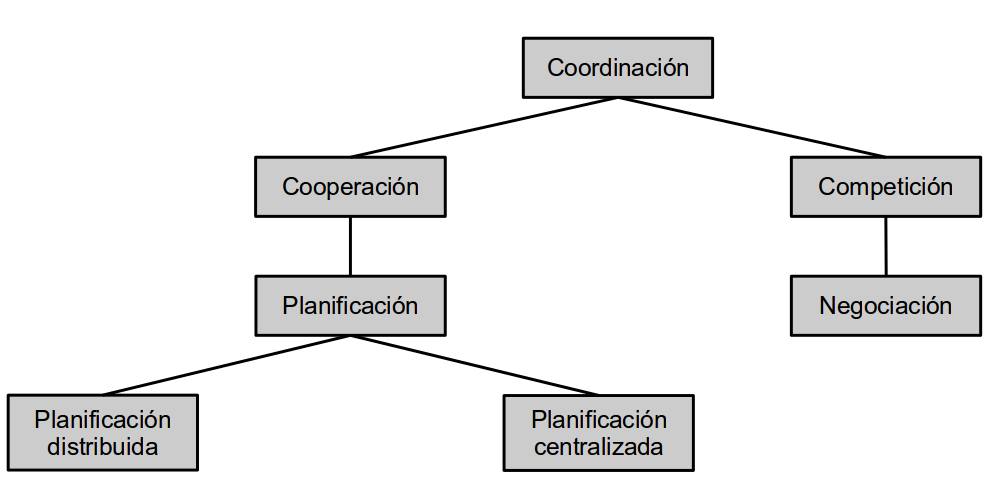
\includegraphics[width=0.8\textwidth]{/coordinacion.png}
\caption[Clasificación de las principales vías de coordinación entre agentes]{Clasificación de las principales vías de coordinación entre agentes \cite{coordinacion2}}
\label{fig:coordinacion}
\end{center}
\end{figure}

Existen tres aspectos principales para estudiar de una manera formal la comunicación entre agentes \cite{coordinacion}: 
\begin{itemize}
\item La \textbf{sintaxis}: cómo se estructuran los símbolos de la comunicación,
\item La \textbf{semántica}: qué significan los símbolos.
\item La \textbf{pragmática}: cómo se interpretan los símbolos.
\end{itemize}

El significado se considera una combinación de la semántica y la pragmática. Los agentes se comunican con el fin de comprender y ser comprendidos, por lo que es importante tener en cuenta las diferentes dimensiones de significado que están asociadas con la comunicación.

«Debido a que normalmente los agentes que forman parte de un mismo sistema multiagente tienen distintas capacidades a la hora de comunicarse,
es importante definir un esquema de comunicación a varios niveles. Normalmente, se identifican distintos roles en una conversación, destacando los de activo, pasivo o ambos. Así mismo, existen dos tipos principales de mensajes (ver Cuadro~\ref{tab:tiposmensaje}): afirmaciones y preguntas» \cite{coordinacion2}.

\begin{table}[htbp]
  \centering
  {\small
  \begin{tabular}{p{.4\textwidth}p{.2\textwidth}p{.2\textwidth}}
  \tabheadformat
  \tabhead{Acto de comunicación} &
  \tabhead{Intención} &
  \tabhead{Resultado deseado} \\
\hline
\textit{Afirmación}  & Informar & Aceptación \\

\hline
\textit{Solicitud}  & Preguntar & Respuesta \\

\hline
\textit{Respuesta}  & Informar & Aceptación \\

\hline
\textit{Solicitud}  & Pedir &  \\

\hline
\textit{Explicación}  & Informar & Acuerdo \\

\hline
\textit{Orden}  & Pedir &  \\

\hline
\textit{Permiso}  & Informar & Aceptación \\

\hline
\textit{Rechazo}  & Informar & Aceptación \\

\hline
\textit{Oferta}  & Informar & Aceptación \\

\hline
\textit{Aceptación}  &  &  \\

\hline
\textit{Acuerdo}  &  &  \\

\hline
\textit{Propuesta}  & Informar & Oferta \\

\hline
\textit{Confirmación}  &  &  \\

\hline
\textit{Retirada}  &  &  \\

\hline
\textit{Denegación}  &  &  \\

\hline
\end{tabular}


% Local variables:
%   coding: utf-8
%   ispell-local-dictionary: "castellano8"
%   TeX-master: "main.tex"
% End:

  }
  \caption[Principales tipos de mensajes entre agentes]
  {Principales tipos de mensajes entre agentes}
  \label{tab:tiposmensaje}
\end{table}
	
\section{Herramientas y entornos de desarrollo}
\label{sec:herrmientas}

En esta sección se analizan los elementos principales escogidos para el desarrollo del proyecto.

\subsection{3DR IRIS+}
\label{sec:3driris}

«El \textbf{3DR IRIS+} (ver Figura~\ref{fig:3dririsplus}) es un vehículo aéreo autónomo todo en uno, producido por 3D Robotics \footnote{\url{https://www.3dr.com}}, que se ejecuta sobre el sistema de piloto automático Pixhawk, lo último en electrónica avanzada para el piloto automático desde el proyecto del PX4. Con la ayuda de puntos \acs{GPS} preprogramados es capaz de efectuar operaciones de nivel profesional, como el mapeo, la toma de imágenes con scripts, la investigación científica, y otras aplicaciones donde se requieren planes de vuelo repetitivos» \cite{3driris}. Es concebido como una plataforma de captación de imágenes aéreas potenciado por hardware, software y firmware de código abierto.

\begin{figure}[!h]
\begin{center}
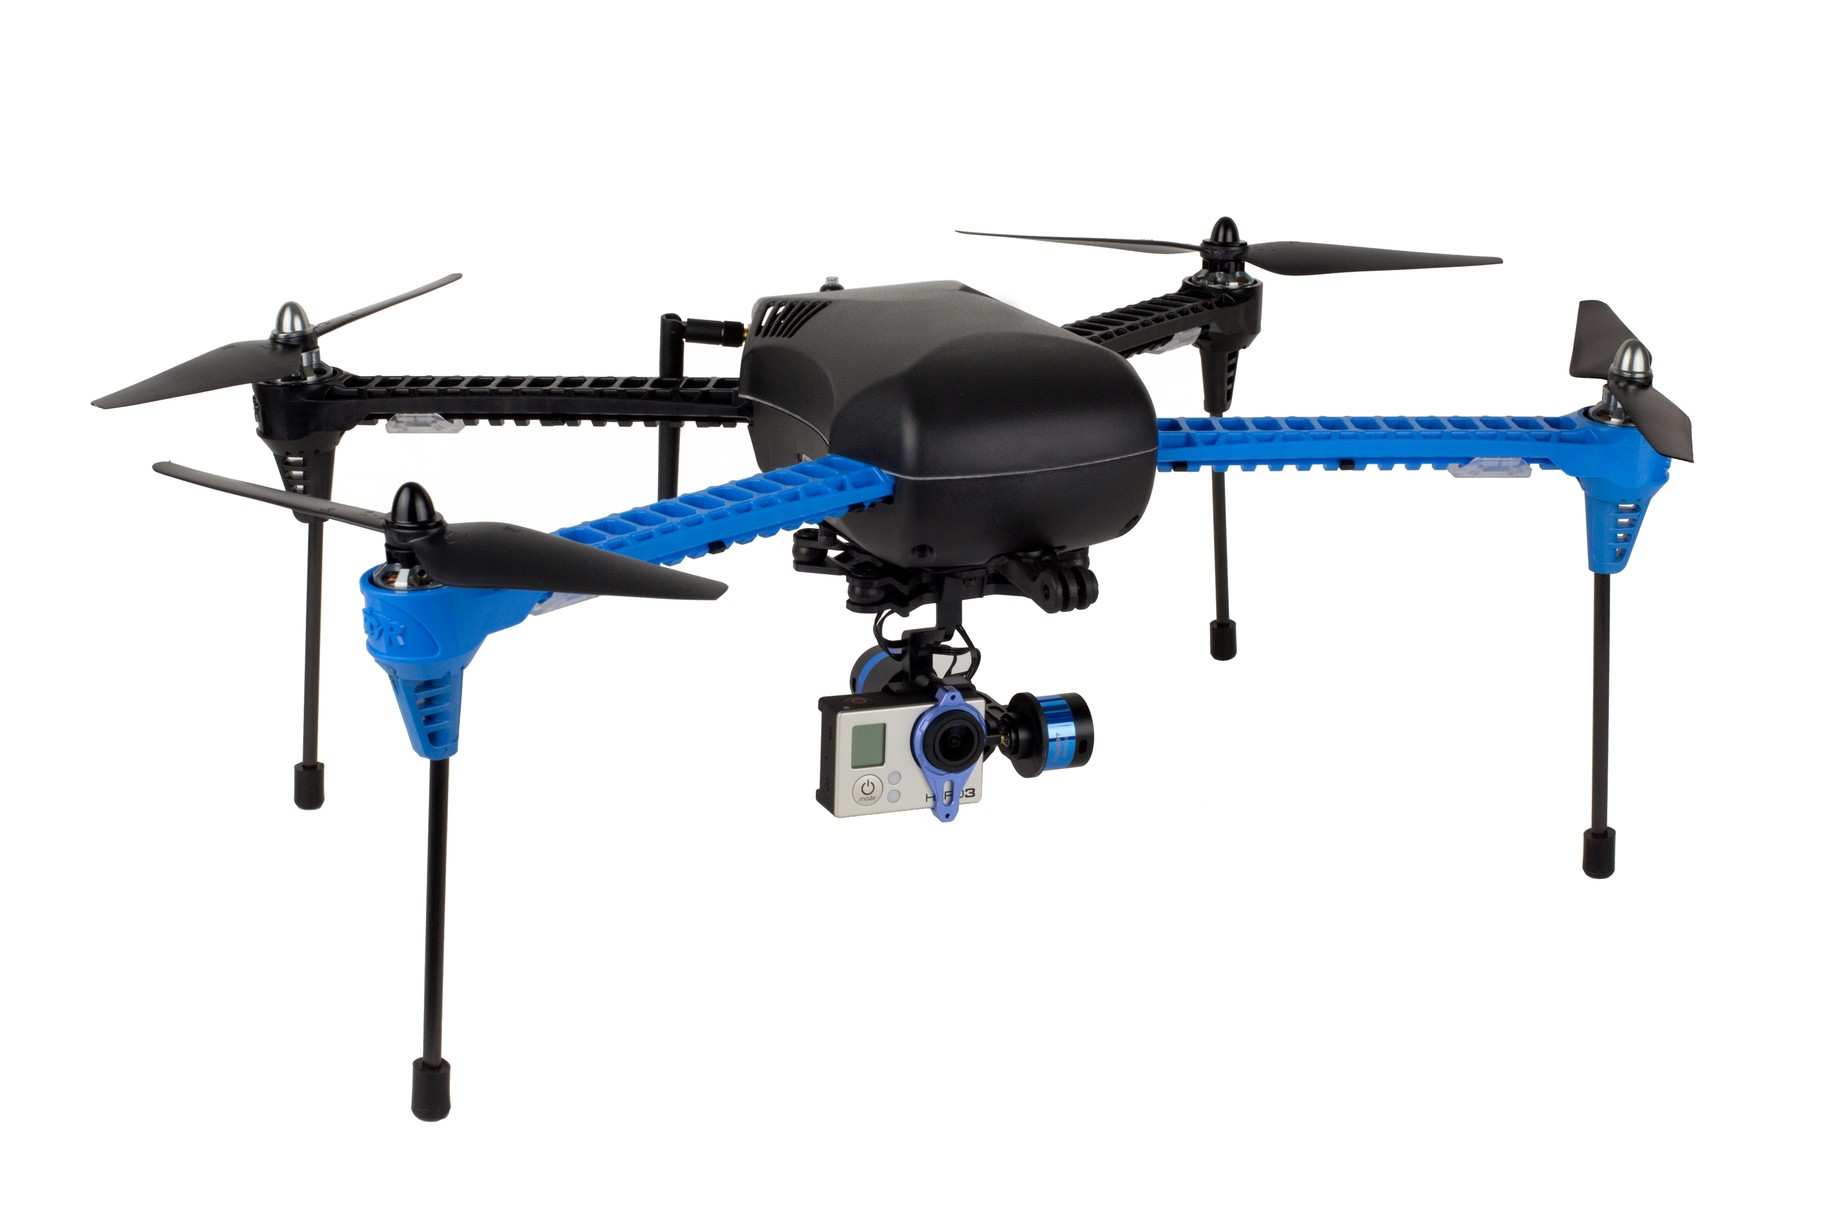
\includegraphics[width=0.8\textwidth]{/3driris.jpg}
\caption[3DR IRIS+]{3DR IRIS+}
\label{fig:3dririsplus}
\end{center}
\end{figure}

El 3DR IRIS+ cuenta con una serie de componentes y especificaciones (ver Cuadro~\ref{tab:especificaciones}) como: GPS integrado, que permite establecer una ruta de antemano o volver a casa en caso de pérdida, o un kit de telemetría que permite obtener información de vuelo como la distancia, altitud, velocidad, nivel de batería e intensidad de la señal \acs{GPS}. Como en cualquier dron, se puede personalizar, y es posible la inclusión de una cámara GoPro Hero si se quiere mejorar la calidad de la imagen.

\begin{table}[htbp]
  \centering
  {\small
  \begin{tabular}{p{.2\textwidth}p{.6\textwidth}}
  \tabheadformat
  \tabhead{Especificaciones} &
  \tabhead{} \\
\hline
\textit{Piloto automático}  & Pixhawk v2.4.5 \\
                 
\hline
\textit{Firmware} &  ArduCopter 3.2 \\
                       
\hline
\textit{GPS}  &  3DR uBlox \acs{GPS} con brújula (módulo LEA-6H) \\
                       
\hline
\textit{Telemetría}  & 3DR Radio Telemetry v2 (433 mHz) \\
                      
\hline
\textit{Motores}  &  MN2213 950 kV (2 unidades en sentido horario y 2 unidades en sentido antihorario) \\
                   
\hline
\textit{Tipo de chasis}  &  V  \\

\hline
\textit{Hélices}  &  9,5 x 4,5 T-Motor multirotor (2 unidades en sentido horario y 2 unidades en sentido antihorario) \\
      
\hline
\textit{Batería}  & Batería de polímero de litio 3S 5,1 Ah 8C \\

\hline
\textit{Voltaje de batería baja}  & 10,5 V \\

\hline
\textit{Máximo voltaje}  & 12,6 V \\

\hline
\textit{Peso de la batería}  & 320 g \\

\hline
\textit{Peso con batería}  & 1282 g \\	

\hline
\textit{Altura}  & 100 mm \\

\hline
\textit{Distancia de motor a motor}  & 550 mm \\

\hline
\textit{Capacidad de carga}  & 400 g  \\

\hline
\textit{Alcance radio}  & Hasta 1 km  \\ 
                
\hline
\end{tabular}


% Local variables:
%   coding: utf-8
%   ispell-local-dictionary: "castellano8"
%   TeX-master: "main.tex"
% End:

  }
  \caption[Especificaciones técnicas del 3DR IRIS+]
  {Especificaciones técnicas del 3DR IRIS+ \cite{especifaciones3dr}}
  \label{tab:especificaciones}
\end{table}

\subsection{ArduPilot}
\label{sec:ardupilot}

\textbf{ArduPilot} \footnote{\url{http://www.ardupilot.com}} es una plataforma de código abierto para pilotos automáticos, de bajo coste y fácil de usar, creada en 2007 por Chris Anderson y Jordi Muñoz, miembros de la comunidad DIY Drones \footnote{\url{http://diydrones.com}}. Se apoya en la plataforma de prototipado electrónico Arduino \footnote{\url{https://www.arduino.cc/}} y es capaz de controlar multirrotores, aeronaves de ala fija, helicópteros tradicionales y vehículos de exploración terrestre. ArduPilot es una plataforma galardonada en 2012 y 2014 en las competiciones UAV Challenge \footnote{\url{https://www.uavchallenge.org}}.

La primera versión de ArduPilot (ver Figura~\ref{fig:APMHistory}), lanzada en 2009, se basó en una termopila, cuya clave era la determinación de la ubicación del horizonte con respecto al avión por la medición de la diferencia de temperatura entre el cielo y el suelo. Más tarde, el sistema se mejoró reemplazando las termopilas con una unidad de medición inercial y utilizando una combinación de acelerómetros, giróscopos y magnetómetros.

\begin{figure}[!h]
\begin{center}
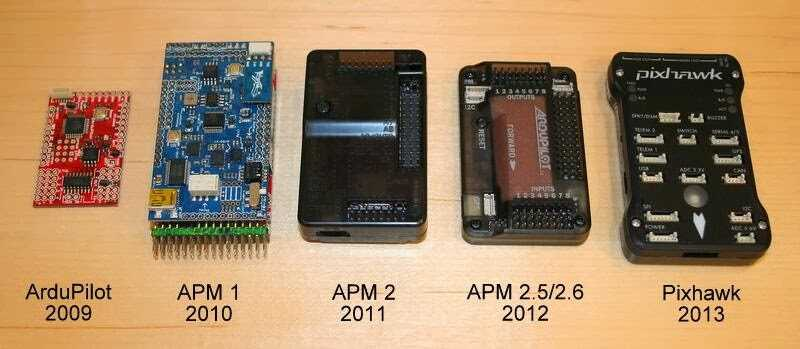
\includegraphics[width=0.8\textwidth]{/APM-history.jpg}
\caption[Historia de ArduPilot]{Historia de ArduPilot \footnotemark}
\label{fig:APMHistory}
\end{center}
\end{figure}

\footnotetext{\url{http://www.ardupilot.org/copter/docs/common-history-of-ardupilot.html}}

En el presente, el proyecto ArduPilot se sustenta sobre cuatro pilares fundamentales:

\begin{itemize}
\item \textbf{Hardware}: Los sistemas embebidos y sensores periféricos que actúan como el cerebro del vehículo, los ojos, las orejas, etc. Entre ellos se encuentra la línea APM y \textbf{Pixhawk}/PX4 de pilotos automáticos.
\item \textbf{Firmware}: El código que implementa el conjunto de habilidades que se ejecuta en el hardware, configurado para el 
tipo de vehículo que se elija. El firmware elegido puede ser \textbf{ArduCopter}(véase \S\,\ref{sec:arducopter}), ArduPlane o ArduRover.
\item \textbf{Software}: La interfaz con el hardware. Por ejemplo, la aplicación de estación de tierra \textbf{Mission Planner}(Anexar documento sobre Mision Planner).
\item \textbf{Comunidad}: Un área para el discurso abierto entre los desarrolladores y sus clientes.
\end{itemize}

El enfoque de ArduPilot respecto a su software libre es que el bajo coste y la disponibilidad permitan el uso en pequeños aviones 
pilotados a distancia.

\subsection{ArduCopter}
\label{sec:arducopter}

«\textbf{ArduCopter} \footnote{\url{http://www.arducopter.co.uk}} es el firmware desarrollado por la comunidad del Proyecto ArduPilot que permite el vuelo, y la monitorización, de aeronaves que basan su funcionamiento, generalmente, en motores eléctricos con hélices  que  ejerzan  la  fuerza  actuadora.  Esta característica  reúne  vehículos  aéreos  como  los  quadrotors, hexarotors, trirotors, octarotors o helicópteros» \cite{arducopter}. Ofrece tanto una experiencia mejorada de vuelo por control remoto como la ejecución de misiones totalmente autónomas.

ArduCopter facilita el uso de \acs{UAV}s, de tipo multirrotor o helicoptero, pudiendo ser ejecutado sobre un piloto automático de ArduPilot.
Junto con el uso de un módulo \acs{GPS}, se convierte en una solución completa que lo diferencia de multirrotores tradicionales que sólo 
soportan el control remoto. El firmware ArduCopter proporciona un vuelo totalmente autónomo basado en «waypoints», a través de 
una estación de control terrestre o \acs{GCS}, que permite la planificación de misiones sirviéndose para ello del empleo de telemetría en tiempo real.

Las principales características que ofrece ArduCopter son las siguientes:
\begin{itemize}
\item \textbf{No requiere conocimientos de programación}: para usar ArduCopter solo se debe descargar una utilidad de escritorio, como 
Mission Planner, que cargue el firmware con un solo clic.
\item Uso de \textbf{puntos de ruta ilimitados}.
\item Permite \textbf{mantener el dron en una localización} determinada valiéndose del \acs{GPS} y del sensor de altitud.
\item \textbf{Vuelta a casa} o \textbf{\acs{RTL}}: ArduCopter establece una posición como punto de despegue, de tal modo, que accionado una palanca el dron regresa automáticamente hasta allí.
\item \textbf{Despegue} y \textbf{aterrizaje automático.}
\item \textbf{Control de la cámara} totalmente programable: incluyendo la capacidad para mantener la cámara apuntando a un objeto en el suelo.
\item \textbf{Multiplataforma}: compatible con Windows, Mac y Linux.
\item \textbf{Compatibilidad con los estándares} de robótica líderes en la industria como el protocolo de comunicación MAVLink \footnote{\url{http://www.qgroundcontrol.org/mavlink/start}}.
\end{itemize}

\subsection{DroneKit-Python}
\label{sec:dronekit}

\textbf{DroneKit-Python} \footnote{\url{http://python.dronekit.io/}} es una \acs{API} desarrollada por 3D Robotics, de código abierto y orientada a la comunidad, que permite crear aplicaciones, para vehículos aéreos no tripulados, que se 
ejecutan en un ordenador. Dichas aplicaciones se comunican con el controlador de vuelo ArduPilot, utilizando un enlace de baja latencia, y pueden mejorar significativamente el piloto automático, añadiendo una mayor inteligencia al comportamiento del vehículo o realizando tareas que son computacionalmente intensivas o sensibles al tiempo (por ejemplo, la visión por ordenador o la planificación de trayectorias).

Se comunica con los vehículos por medio del protocolo \textbf{MAVLink}. Proporciona acceso, mediante programación, a la información 
de telemetría, al estado y parámetros de información del vehículo, y permite gestionar las misiones y tener un control directo 
sobre el vehículo. Se ejecuta en Linux, Mac OS X o Windows.

Dronekit-Python proporciona clases y métodos para realizar múltiples funciones, entre otras:
\begin{itemize}
\item \textbf{Conexión} a uno o varios \textbf{vehículos}.
\item \textbf{Obtener y establecer información} sobre el estado del vehículo.
\item Recibir \textbf{notificaciones} asíncronas de los \textbf{cambios de estado}.
\item \textbf{Guiar} un \textbf{\acs{UAV}} hasta una posición especificada.
\item Crear y \textbf{gestionar misiones} gracias a «waypoints».
\item \textbf{Reemplazar} la configuración de los \textbf{canales de radiocontrol}.
\end{itemize}

«Cuando DroneKit no proporciona un comando para una maniobra deseada, se requiere el uso de mensajes personalizados MAVLink.
Cualquier maniobra aérea debe ser capaz de llevarse a cabo a través de una de estas dos interfaces» \cite{dronekit}. 

(Posible anexo sobre buenas practicas propuestas por dronekit)

\subsection{OpenCV}
\label{sec:opencv}

\textbf{OpenCV} \footnote{\url{http://www.opencv.org}} es una biblioteca de funciones de programación, para la visión por computador 
en tiempo real, iniciado en Intel en 1999 por Gary Bradsky. Se encuentra bajo licencia BSD, por lo tanto, es libre tanto en el uso
académico como en el comercial. Posee interfaces en C++, C, Python y Java, y es compatible con Windows, Linux, Android, iOS y Mac OS.
Cuenta con más de 2500 algoritmos optimizados y más de 9 millones de descargas.

«La librería OpenCV está dirigida fundamentalmente a la visión por computador en tiempo real. Entre sus muchas áreas de 
aplicación destacarían: interacción hombre-máquina, segmentación y reconocimiento de objetos, reconocimiento de gestos, 
seguimiento del movimiento, estructura del movimiento y robots móviles» \cite{opencv}.

El  conjunto  de  funciones   suministradas por la librería OpenCV se agrupan en los siguientes bloques: 
\begin{itemize}
\item Estructuras y \textbf{operaciones básicas}: matrices, grafos, árboles, etc.
\item Procesamiento y \textbf{análisis de imágenes}: filtros, momentos, histogramas, etc.
\item \textbf{Análisis estructural}: geometría, procesamiento del contorno, etc.
\item \textbf{Análisis del movimiento} y \textbf{seguimiento de objetos}: plantillas  de  movimiento, seguidores, flujo óptico, etc.
\item \textbf{Reconocimiento de objetos}: objetos propios, modelos \acs{HMM}, etc.
\item \textbf{Calibración de la cámara}: morphing, geometría epipolar, estimación de la pose, etc.
\item \textbf{Reconstrucción tridimensional}: detección de objetos, seguimiento de objetos tridimensionales, etc.
\item Interfaces gráficos de usuarios y \textbf{adquisición de video}.
\end{itemize}

\subsection{Google Cloud Vision API}
\label{sec:visionapi}

\textbf{Google Cloud Vision API} \footnote{\url{https://cloud.google.com/vision/}} permite a los desarrolladores entender el contenido de una imagen, mediante la encapsulación de potentes modelos de aprendizaje automático. Esta REST API clasifica rápidamente las imágenes en miles de categorías, detecta objetos individuales y caras, y encuentra y lee palabras impresas.

Es capaz de detectar conjuntos de objetos en las imágenes, como flores, automóviles, animales u otros de los muchos elementos 
que se encuentran comúnmente dentro de las fotografías. También, puede analizar atributos faciales emocionales de las personas en sus imágenes, como la alegría, la tristeza y la ira. Se encuentra en constante progreso a medida que se introducen nuevos conceptos y se mejora la precisión.

Vision API ofrece las siguientes funcionalidades:
\begin{itemize}
\item \textbf{Detección de etiquetas}: detecta amplios conjuntos de categorías.
\item \textbf{Detección de rostros}: detección de múltiples caras, junto con los atributos faciales claves asociados.
\item \textbf{Detección de contenido explícito}: detecta contenido explícito como contenido para adultos o de contenido violento.
\item \textbf{Atributos de imagen}: detecta los atributos generales de la imagen, como el color dominante.
\item \textbf{Detección de logotipos} populares.
\item \textbf{Detección de interés}: detección de estructuras naturales y artificiales populares.
\item \textbf{Reconocimiento óptico de caracteres}: detecta y extrae el texto, con soporte para una amplia gama de idiomas, junto con el soporte para la identificación automática del lenguaje.
\item \textbf{REST API integrada}: acceso a través de la REST API para solicitar uno o más tipos de detección por imagen.
\end{itemize}

El uso de cada una de estas características conlleva gastos.

\section{Sistemas para catástrofes}
\label{sec:sistemas}

La alta frecuencia de desastres, tanto naturales como artificiales, que puedan causar la perdida de seres humanos, son un problema en el que los drones pueden contribuir a una notable mejoría en los tiempos de respuesta y actuación.

Un grupo multidisciplinar de voluntariado con equipos de alta tecnología puede ayudar a conservar la vida de una persona o a realizar un análisis más rápido en situaciones de emergencia, en las cuales pueden correr peligro, no ya una, sino cientos de vidas. Es evidente que visión global aérea de un cataclismo puede brindar la posibilidad de tomar decisiones más correctas.

Si algo ha cambiado rápido en estos últimos tiempos es la visión popular a cerca de los drones. Hoy es muy habitual que quien observa el vuelo de un dron se pregunte si está prohibido hacerlo (Anexar normativa de vuelo de drones). Y es que parece ser que se está estigmatizando esta herramienta cuyas capacidades son tan beneficiosas que deberían despejar las dudas sobre la legalidad de su manejo.

El despliegue de esta tecnología supone un cambio radical en labores de ayuda y rescate de vidas humanas, desde el posicionamiento óptimo, la logística y aporte de medios, hasta el rescate de vidas en sí mismo.

Los drones, a diferencia que una UVI móvil, no pueden atender al paciente en movimiento durante su traslado con la participación de varios doctores. Pero sí que es posible el transporte urgente y existen proyectos para el envío de un dron que pueda portar un desfibrilador \footnote{\url{http://www.io.tudelft.nl/onderzoek/delft-design-labs/applied-labs/ambulance-drone/}} (ver Figura~\ref{fig:ambulancedrone}).

\begin{figure}[!h]
\begin{center}
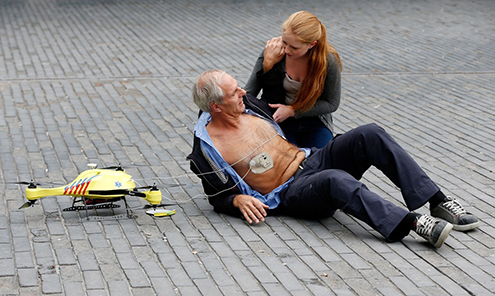
\includegraphics[width=0.8\textwidth]{/ambulancedrone.jpg}
\caption[Ambulance Drone]{Ambulance Drone}
\label{fig:ambulancedrone}
\end{center}
\end{figure}

«Los drones de rescate han entrado en acción en zonas de contaminación, tras un accidente nuclear, en terremotos o inundaciones. Son pequeños y pueden buscar personas y objetos en grandes áreas, incluso de noche. Consiguen imágenes accediendo a edificios a punto de caer, buscando supervivientes y obteniendo datos e información vital. Son capaces de realizar vuelos entre el humo de los incendios e identifican térmicamente siluetas de personas para saber dónde están atrapados o si se han desmayado y están inconscientes. En atmósferas explosivas y tras accidentes por explosión de gas, inspeccionan y toman muestras del aire, pasan entre los escombros localizando a las personas, se mueven rápido y pueden recoger muestras de agua contaminada o sustancias químicas tras acceder a sitios inverosímiles. Y todo ello en apenas unos minutos, visualmente, y en tiempo real, enviándolo al instante a los centros de control, mejorando así los resultados y disminuyendo los costes» \cite{dron3}.

En resumen, es posible concebir un futuro muy próximo con aplicaciones en las que los ciudadanos tengan la seguridad de poder solicitar y contar con un dron ante cualquier situación de necesidad, urgencia y de peligro.

\subsection{Proyecto ICARUS}
\label{sec:icarus}

Después de los terremotos en L'Aquila, Haití y Japón, la Comisión Europea confirmó que existe una gran discrepancia entre la tecnología, que se desarrolla en el laboratorio, y el uso de dicha tecnología, en el terreno para las operaciones de búsqueda y rescate (\acs{ByR}) y la gestión de crisis.

De este modo, la Dirección General de Empresa e Industria de la Comisión Europea decidió financiar ICARUS \footnote{\url{http://www.fp7-icarus.eu/}}, un proyecto de investigación, con un presupuesto total de 17,5 millones de euros, que tiene como objetivo desarrollar herramientas robóticas pueden ayudar a los equipos de intervención en situaciones de crisis.

La introducción de dispositivos no tripulados, en misiones de \acs{ByR}, pueden ofrecer una herramienta de valor para salvar vidas humanas y para acelerar el proceso de \acs{ByR}. ICARUS se concentra en el desarrollo de las tecnologías de búsqueda y rescate, con \acs{UAV}s, para la detección, localización y el rescate de seres humanos.

Existe una amplia literatura sobre los esfuerzos de investigación hacia el desarrollo de herramientas de \acs{ByR}. Sin embargo, este esfuerzo de investigación está en contraste con la realidad práctica en el campo, donde herramientas de búsqueda y salvamento no tripuladas tienen grandes dificultades para encontrar a usuarios finales. El proyecto ICARUS se ocupa de estos problemas, con el objetivo de cerrar la brecha entre la comunidad científica y los usuarios finales.

El objetivo general del proyecto ICARUS es aplicar sus innovaciones para la mejora de la gestión de una crisis y de este modo, reducir el riesgo y el impacto de la crisis sobre los ciudadanos. 

El uso de dispositivos no tripulados de \acs{ByR}, embebidos en una arquitectura apropiada e integrados en las infraestructuras existentes, ayudarán al personal de crisis, proporcionando información detallada y fácil de entender sobre la situación. El sistema propuesto debe informar al personal de crisis sobre los peligros reales presentes en el suelo, y por lo tanto aumentará su rendimiento en la resolución de la situación.

\subsection{Sistema Pelícano}
\label{sec:pelicano}

El sistema Pelícano de Indra \footnote{\url{http://www.indracompany.com/es/}} (ver Figura~\ref{fig:pelicano}), está formado por cuatro helicópteros no tripulados y una estación de control, que proporciona capacidad para operar las 24 horas del día durante periodos prolongados. Su diseño ha sido pensado para responder a los requisitos y necesidades de las fuerzas armadas y de seguridad.

\begin{figure}[!h]
\begin{center}
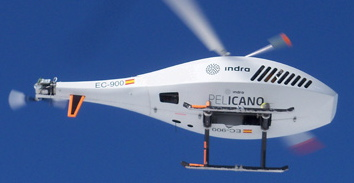
\includegraphics[width=0.8\textwidth]{/indra-pelicano.jpg}
\caption[\acs{UAV} Pelícano de Indra]{\acs{UAV} Pelícano de Indra}
\label{fig:pelicano}
\end{center}
\end{figure}

El sistema de \acs{UAV}s Pelícano \cite{PELICANO} esta preparado para dar apoyo, tanto en misiones de inteligencia como en gestión de emergencias, tales como 
desastres naturales o medioambientales, que impliquen el seguimiento, vigilancia y reconocimiento de amplias superficies, eliminando así pérdidas humanas.

Indra ha basado el sistema en un helicóptero de tamaño medio de la compañía sueca CybAero e incorporará los sistemas tecnológicos más avanzados para adaptarlo a las necesidades operativas militares y civiles. 

Entre los sensores con que está dotada la aeronave figuran sistemas electro-ópticos de visión diurna e infrarroja, capaces de tomar imágenes de muy alta resolución  a gran altura. También esta acondicionado para poder portar un radar ligero, así como sistemas de inteligencia electrónica y sensores de detección de amenazas químicas, bacteriológicas, radioactivas y nucleares.

\subsection{Proyecto ATLANTE}
\label{sec:atlante}

El Centro para el Desarrollo Tecnológico Industrial (CDTI) actuó como organismo gestor de programas del sector aeronáutico, y lanzó el programa \acs{ATLANTE}, liderado por Cassidian, tras constatar el interés de la Industria española por los \acs{UAS} y con el fin de potenciar el desarrollo de la tecnología asociada a este tipo de sistemas mediante un proyecto realizado íntegramente en España.

El \acs{ATLANTE} (ver Figura~\ref{fig:atlante}) es un sistema diseñado para responder a las necesidades de las fuerzas terrestres militares desplegadas en el teatro de operaciones, que les permite realizar misiones de inteligencia, vigilancia y reconocimiento de día y noche en condiciones climatológicas adversas. También permite llevar a cabo labores de identificación de blancos, corrección de tiro y evaluación de daños.

\begin{figure}[!h]
\begin{center}
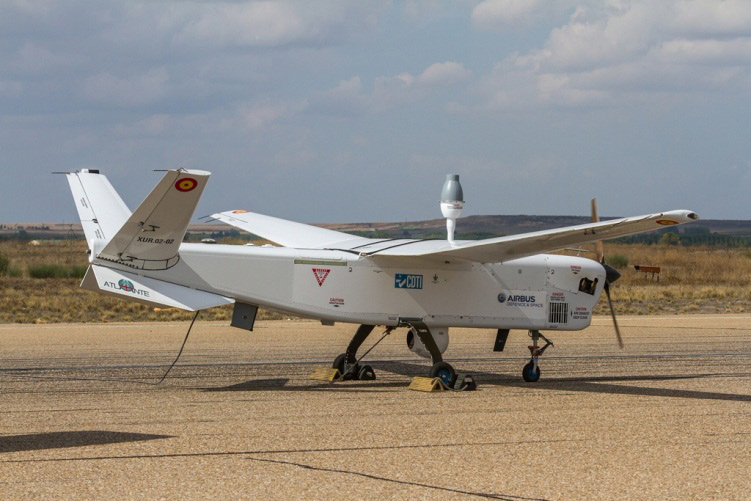
\includegraphics[width=0.8\textwidth]{/atlante.jpg}
\caption[\acs{UAV} \acs{ATLANTE}]{\acs{UAV} \acs{ATLANTE}}
\label{fig:atlante}
\end{center}
\end{figure}

El sistema está formado por cuatro o más vehículos aéreos no tripulados, una estación de control terrestre, una unidad de transporte, lanzamiento y recogida y terminales de video remoto. Los equipos de misión de la plataforma aérea recogen la información de los sensores y los transmite a tierra mediante los enlaces de datos de alta velocidad para su posterior explotación.

Como características principales de sistema cabe destacar la facilidad de despliegue por tierra, mar y aire, y el despegue y aterrizaje tanto en pistas convencionales como no preparadas, así como el despegue fuera de pistas mediante catapulta neumática y la recuperación mediante paracaídas.

Entre las aplicaciones no militares estarían las orientadas hacia la lucha anti-terrorista y contra la piratería, control de inmigración ilegal y tráfico de drogas y, cómo no, para la lucha contra incendios y otros desastres naturales y supervisión de infraestructuras críticas y vías de comunicación.


% Local Variables:
%  coding: utf-8
%  mode: latex
%  mode: flyspell
%  ispell-local-dictionary: "castellano8"
% End:
